\chapter{Linear Algebra}
\section{Linear Vector Space}
\subsection{Definition}
\begin{newdef}[Linear vector space]
A linear vector space is a set of elements, called vectors, which is closed under addition and multiplication by scalars. That is to say, if $\phi$ and $\psi$ are vectors then so is $a\phi+b\psi$, where $a$ and $b$ are arbitrary scalars. If the scalars belong to the field of complex (real) numbers, we speak of a complex (real) linear vector space. Henceforth the scalars will be complex numbers unless otherwise stated.
\end{newdef}

\begin{example}
\begin{enumerate}
\item Discrete vectors, which may be represented as columns of complex numbers.
\item Spaces of functions of some type, for example the space of all differentiable functions
\end{enumerate}
\end{example}

\subsection{Linear independence}
\begin{newdef}[Linear independence]
A set of vectors $\{\phi_n\}$ is said to be linearly independent if no non-trivial linear combination of them sums to zero; that is to say, if the equation $\sum_{n} c_n \phi_n$ can hold only when $c_n=0$ for all $n$. If this condition does not hold, the set of vectors is said to be linearly dependent, in which case it is possible to express a member of the set as a linear combination of the others.
\end{newdef}

\begin{newdef}[Dimension]
The maximum number of linearly independent vectors in a space is called the dimension of the space.
\end{newdef}

\begin{newdef}[Base]
A maximal set of linearly independent vectors is called a basis for the space. Any vector in the space can be expressed as a linear combination of the basis vectors.
\end{newdef}

\subsection{Inner product}
\begin{newdef}[Inner product]
An inner product (or scalar product) for a linear vector space associates a scalar $(\phi,\psi)$ with every ordered pair of vectors. 
It must satisfy the following properties:
\begin{enumerate}
\item $(\phi,\psi) = $ a complex number.
\item $(\phi,\psi) = (\psi,\phi)^*$.
\item $(\phi,c_1\psi_1 + c_2\psi_2) = c_1(\phi,\psi_1) + c_2(\phi,\psi_2)$.
\item $(\phi,\phi) \geq 0$,with equality holding if and only if $\phi=0$.
\end{enumerate}
\end{newdef}

\begin{example}
\begin{enumerate}
\item If $\psi$ is the column vector with elements $a_1$, $a_2$, $\cdots$, and $\phi$ is the column vector with elements $b_1$, $b_2$, $\cdots$, then
\[(\psi,\phi) = a_1^*b_1 + a_2^*b_2 + \cdots\]
\item If $\psi$ and $\phi$ are functions of $x$, then
\[(\phi,\psi) = \int \phi^*(x) \psi(x) w(x) dx,\]
where $w(x)$ is some non-negative weight function.
\end{enumerate}
\end{example}

\begin{newdef}[Norm]
\[|| \phi || \equiv (\phi,\phi)^{\frac{1}{2}}.\]
\end{newdef}

\begin{newthem}[Schwarz's inequality]
\[|(\psi,\phi)|^2 \leq (\psi,\psi)(\phi,\phi).\]
\end{newthem}

\begin{newthem}[triangle inequality]
\[||(\psi+\phi)|| \leq ||\phi|| + ||\psi||.\]
\end{newthem}

\begin{newdef}[Orthonormal]
A set of vectors $\{\phi_n\}$ is said to be orthonormal if the vectors are pairwise orthogonal and of unit norm; that is to say, their inner products satisfy $(\psi_m,\phi_n) = \delta_{mn}$.
\end{newdef}

\subsection{Dual space}
\begin{newdef}[Dual vector]
Corresponding to any linear vector space $V$ there exists the dual space of linear functionals on $V$ . A linear functional $F$ assigns a scalar $F(\phi)$ to each vector $\phi$, such that
\[F(a\phi+b\psi) = aF(\phi) + bF(\psi) \]
for any vectors for $\phi$ and $\psi$, and any scalars $a$ and $b$. The set of linear functionals may itself be regarded as forming a linear space $V'$ if we define the sum of two functionals as
\[(F_1+F_2)(\phi) \equiv F_1(\phi) + F_2(\phi).\]
\end{newdef}

\begin{newthem}[Riesz theorem] 
There is a one-to-one correspondence between linear functionals $F$ in $V'$ and vectors $f$ in $V$, such that all linear functionals have the form
\[F(\phi) = (f,\phi),\]
$f$ being a fixed vector, and $\phi$ being an arbitrary vector. Thus the spaces $V$ and $V'$ are essentially isomorphic.
\end{newthem}

\subsection{Dirac's bra and ket notation}
\noindent
In Dirac's notation, which is very popular in quantum mechanics, the vectors in $V$ are called ket vectors, and are denoted as $|\phi \rangle$. The linear functionals in the dual space $V'$ are called bra vectors, and are denoted as $\langle F |$. The numerical value of the functional is denoted as
\[F(\phi) = \langle F | \phi \rangle.\]
According to the Riesz theorem, there is a one-to-one correspondence between bras and kets. Therefore we can use the same alphabetic character for the functional (a member of $V'$) and the vector (in $V$ ) to which it corresponds, relying on the bra, $\langle F |$, or ket, $|F\rangle$, notation to determine which space is referred to. Thus
\[\langle F | \phi \rangle = (F,\phi).\]
Note that the Riesz theorem establishes, by construction, an antilinear correspondence between bras and kets. If $\langle F | \leftrightarrow  |F\rangle$, then
\[c_1^* \langle F_1 | + c_2^* \langle F_2 | \leftrightarrow  c_1 |F_1\rangle + c_2|F_2\rangle.\]

\section{Linear Operators}
\begin{newdef}[Linear operators]
An operator on a vector space maps vectors onto vectors.
A linear operator satisfies
\[A (c_1 \psi_1 + c_2 \psi_2) = c_1 A(\psi_1) + c_2 A(\psi_2).\]
Define the sum and product of operators,
\begin{eqnarray}
(A+B)\psi &\equiv & A\psi + B\psi, \nonumber \\
A B \psi &\equiv & A (B\psi). \nonumber
\end{eqnarray}
Define their action to the left on bra vectors as
\[(\langle \phi | A ) \psi \rangle \equiv \langle \phi | ( A | \psi \rangle ).\]
Thus we may define the operation of $A$ on the bra space of functionals as
\[A F_{\phi} (\psi) \equiv F_{\phi}(A\psi).\]
According to the Riesz theorem there must exist a ket vector $\chi$ such that
\[AF_{\phi}(\psi) = (\chi, \psi) = F_{\chi}(\psi).\]
Define operator $A^{\dagger}$ as
\[AF_{\phi} = F_{A^{\dagger}\chi}.\]
Therefore,
\[(A^{\dagger}\phi, \psi) = (\phi, A\psi),\]
\[\langle \psi | A^{\dagger} | \phi \rangle ^* = \langle \phi | A | \psi \rangle.\]
\end{newdef}

\begin{newdef}[Outer product]
\[(| \psi \rangle \langle \phi |) | \lambda \rangle \equiv | \psi \rangle (\langle \phi | \lambda \rangle).\]
\end{newdef}

\begin{newdef}[Trace]
\[ \mathrm{Tr} A \equiv \sum \langle u_j | A | u_j \rangle ,\]
where $\{ u_j \}$ may be any orthonormal basis. It can be shown that the value of $\mathrm{Tr}A$ is independent of the particular orthonormal basis that is chosen for its evaluation.
\end{newdef}

\begin{newprop}
\begin{eqnarray}
(cA)^{\dagger} &=& c^* A^{\dagger} .\nonumber \\
(A + B)^{\dagger} &=& A^{\dagger} + B^{\dagger} .\nonumber \\
(AB)^{\dagger} &=& B^{\dagger}  A^{\dagger} .\nonumber
\end{eqnarray}
\[(| \psi \rangle \langle \phi |) ^ {\dagger} = | \phi \rangle \langle \psi |.\]
\end{newprop}

\section{Self-Adjoint operators}
\begin{newdef}[Self-Adjoint operators]
An operator $A$ that is equal to its adjoint $A^{\dagger}$ is called self-adjoint. This means that it satisfies
\[\langle \phi | A | \psi \rangle  = \langle \psi | A | \phi \rangle^* \]
and that the domain of $A$ coincides with the domain of $A^{\dagger}$. An operator that only satisfies above equation is called Hermitian.
\end{newdef}

\begin{newthem}
If $\langle \psi | A | \psi \rangle  = \langle \psi | A | \psi \rangle^*$ for all $| \psi \rangle$, then it follows that $\langle \phi_1 | A | \phi_2 \rangle  = \langle \phi_2 | A | \phi_1 \rangle^*$ for all $|\phi_1\rangle$ and $|\phi_2\rangle$, and hence that $A = A^{\dagger}$.\\
If an operator acting on a certain vector produces a scalar multiple of that same vector,
\[ A |\phi \rangle = a |\phi \rangle,\]
we call the vector $| \phi \rangle$ an eigenvector and the scalar an eigenvalue of the operator $A$. The antilinear correspondence between bras and kets, and the definition of the adjoint operator $A^{\dagger}$, imply that the left-handed eigenvalue equation
\[\langle \phi | A^{\dagger} = a^{*} \langle \phi |.\]
\end{newthem}

\begin{newthem}
 If $A$ is a Hermitian operator then all of its eigenvalues are real.
\end{newthem}

\begin{newthem}
Eigenvectors corresponding to distinct eigenvalues of a Hermitian operator must be orthogonal.
\end{newthem}

\noindent
If the orthonormal set of vectors $\{ \phi_i \}$ is complete, then we can expand an arbitrary vector $|v\rangle$ in terms of it:
\[ |v\rangle = \sum | \phi_i \rangle (\langle \phi_i | v \rangle) = \left( \sum |\phi_i \rangle \langle \phi_i | \right) | v\rangle.\]
Therefore,
\[ \sum |\phi_i \rangle \langle \phi_i | = I.\]
If $A |\phi_i \rangle = a_i |\phi_i\rangle$ and the eigenvectors form a complete orthonormal set, then the operator can be reconstructed in a useful diagonal form in terms of its eigenvalues and eigenvectors:
\[A = \sum a_i |\phi_i \rangle \langle \phi_i |.\]
We can define a function of an operator
\[f(A) =  \sum f(a_i) |\phi_i \rangle \langle \phi_i |.\]
The Hermitian operators in a finite N-dimensional vector space have complete sets of eigenvectors. But This statement does not carry over to infinite-dimensional spaces. A Hermitian operator in an infinite dimensional vector space may or may not possess a complete set of eigenvectors, depending upon the precise nature of the operator and the vector space. Instead, we have spectral theorem.

\begin{newthem}
To each self-adjoint operator $A$ there corresponds a unique family of projection operators, $E(\lambda)$, for real $\lambda$, with the properties:
\begin{enumerate}
\item If $\lambda_1 < \lambda_2$ then $E(\lambda_1)E(\lambda_2) = E(\lambda_2)E(\lambda_1)= E(\lambda_1) $.
\item If $\epsilon > 0$, then $E(\lambda + \epsilon)|\psi\rangle \to E(\lambda)|\psi\rangle$ as $\epsilon \to 0$.
\item $E(\lambda)|\psi\rangle \to 0$ as $\lambda \to -\infty$.
\item $E(\lambda)|\psi\rangle \to |\psi\rangle$ as $\lambda \to \infty$.
\item $\int_{-\infty}^{\infty} \lambda dE(\lambda) = A$.
\end{enumerate}
\end{newthem}

\noindent
We can define a function of an operator
\[f(A) = \int_{-\infty}^{\infty} f(\lambda) dE(\lambda).\]
Following Dirac's pioneering formulation, it has become customary in
quantum mechanics to write a formal eigenvalue equation for an operator such as $Q$ that has a continuous spectrum,
\[Q |q\rangle = q|q\rangle.\]
The orthonormality condition for the continuous case takes the form
\[\langle q' | q'' \rangle = \delta(q-q').\]
Evidently the norm of these formal eigenvectors is infinite, since 
$\langle q | q \rangle \to \infty$. Instead of the spectral theorem for $Q$, Dirac would write
\[Q = \int_{-\infty}^{\infty} q |q\rangle\langle q| dq.\]
Dirac's formulation does not fit into the mathematical theory of Hilbert space, which admits only vectors of finite norm. The projection operator formally given by
\[E(\lambda) = \int_{-\infty}^{\lambda}  |q\rangle\langle q| dq \]
is is well defined in Hilbert space, but its derivative does not exist within the Hilbert space framework.\\


\begin{newthem}
If $A$ and $B$ are self-adjoint operators, each of which possesses a complete set of eigenvectors, and if $AB =BA$, then there exists a complete set of vectors which are eigenvectors of both $A$ and $B$.
\end{newthem}

\noindent
Let $(A, B, \cdots)$ be a set of mutually commutative operators that possess a complete set of common eigenvectors. Corresponding to a particular eigenvalue for each operator, there may be more than one eigenvector. If, however, there is no more than one eigenvector (apart from the arbitrary phase and normalization) for each set of eigenvalues $(a_n, b_m, \cdots)$, then the operators $(A, B, \cdots)$ are said to be a complete commuting set of operators.\\


\begin{newthem}
Any operator that commutes with all members of a complete commuting set must be a function of the operators in that set.
\end{newthem}

\section{Rigged Hilbert space}
\begin{newdef}[Rigged Hilbert spece]
Formally, a rigged Hilbert space consists of a Hilbert space $\mathcal{H}$, together with a subspace $\Phi$ which carries a finer topology, that is one for which the natural inclusion $\Phi \subseteq \mathcal{H}$ is continuous. 
It is no loss to assume that $\Phi$ is dense in $\mathcal{H}$ for the Hilbert norm. We consider the inclusion of conjugate space $\mathcal{H}^{\mathrm{X}}$ in $\Phi^{\mathrm{X}}$. $\Phi^{\mathrm{X}}$ is the space of $\tau_{\Phi}$ continuous antilinear functional on $\Phi$.\\
For any $\phi \in \Phi$, $F \in \Phi^{\mathrm{X}}$,we define
\[\langle \phi | F \rangle \equiv F(\phi),\]
\[\langle F | \phi \rangle \equiv [F(\phi)]^*.\]
Now by applying the Riesz representation theorem we can identify $\mathcal{H}^{\mathrm{X}}$ with $\mathcal{H}$. Therefore, the definition of rigged Hilbert space is in terms of a sandwich:
\[\Phi \subseteq \mathcal{H} \subseteq \Phi^{\mathrm{X}}.\]
\end{newdef}

\noindent
There may or may not exist any solutions to the eigenvalue equation $A|a_n\rangle = a_n |a_n\rangle$ for a self-adjoint operator $A$ on an infinite-dimensional vector space. However, the generalized spectral theorem asserts that if $A$ is self-adjoint in $\mathcal{H}$ then a complete set of eigenvectors exists in the extended space $\Phi^{\mathrm{X}}$. The precise conditions for the proof of this theorem are rather technical, so the interested reader is referred to \emph{Gel'fand and Vilenkin (1964)} for further details.
\\
There are many examples of rigged-Hilbert-space triplets. A Hilbert space $\mathcal{H}$ is formed by those functions that are square-integrable. That is, $\mathcal{H}$ consists of those functions $\psi(x)$ for which
\[\langle \psi | \psi \rangle = \int_{-\infty}^{\infty} |\psi(x)|^2 dx \mbox{ is finite }.\]
A nuclear space $\Phi$ is made up of functions $\psi(x)$ which satisfy the infinite set of conditions,
\[\ \int_{-\infty}^{\infty} |\psi(x)|^2(1+|x|)^m dx \mbox{ is finite for } m = 0,1,2,\cdots \]
The functions $\psi(x)$) which make up $\Phi$ must vanish more rapidly than any inverse power of $x$ in the limit $|x| \to \infty$. The extended space $\Phi^{\mathrm{X}}$, which is conjugate to $\Phi$, consists of those functions $\chi(x)$ for which
\[\langle \chi | \psi \rangle = \int_{-\infty}^{\infty} \chi^*(x)\psi(x) dx \mbox{ is finite for any } \psi \mbox{ in } \Phi.\]
\\
In addition to the functions of finite norm, which also lie in $\mathcal{H}$, $\Phi^{\mathrm{X}}$ will contain functions that are unbounded at infinity provided the divergence is no worse than a power of $x$. Hence $\Phi^{\mathrm{X}}$ contains $e^{ikx}$, which is an eigenfunction
of the operator $D = i \frac{d}{dx}$. It also contains the Dirac delta function, $\delta(x-\lambda)$, which is an eigenfunction of the operator $X$, defined by $X\psi(x) = x\psi(x)$.
These two examples suffice to show that rigged Hilbert space seems to be a more natural mathematical setting for quantum mechanics than is Hilbert space.

\section{Unitary operators}
\begin{newdef}[Unitary operator]
 A unitary operator is a bounded linear operator $U: H\to H$ on a Hilbert space $H$ that satisfies $UU^{\dagger} = U^{\dagger}U =I$, where $U^{\dagger}$ is the adjoint of $U$, and $I: H \to H$ is the identity operator.
\end{newdef}
\noindent
Consider a family of unitary operators, $U(s)$, that depend on a single continuous parameter $s$. 
Let $U(0) = I $ be the identity operator, and let $U(s_1+s_2) = U(s_1)U(s_2)$.
We can demonstrate that
\[\left. \frac{dU}{ds}\right|_{s=0} = iK \mbox{ with } K = K^{\dagger}.\]
The Hermitian operator $K$ is called the generator of the family of unitary operators because it determines $U(s)$, not only for infinitesimal $s$, but for all $s$. This can be shown by differentiating
\[U(s_1+s_2) = U(s_1)U(s_2) \]
with respect to $s_2$ and we can get
\[\left. \frac{dU}{ds}\right|_{s=s_1} = U(s_1)iK .\]
This first order differential equation with initial condition $U(0) = I$ has the unique solution
\[U(s) = e^{iKs}.\]

\section{Antiunitary operators}
\begin{newdef}[Antiunitary operator]
In mathematics, an antiunitary transformation, is a bijective antilinear map
\[U:H_{1}\to H_{2} \]
between two complex Hilbert spaces such that
\[\langle Ux,Uy\rangle ={\overline {\langle x,y\rangle }} \]
for all $x$ and $y$ y in $H_{1}$, where the horizontal bar represents the complex conjugate. If additionally one has $H_{1}=H_{2}$ then $U$ is called an antiunitary operator.
\end{newdef}

\begin{newprop}
\begin{enumerate}
\item $\langle Ux,Uy\rangle =\overline {\langle x,y\rangle }=\langle y,x\rangle$ holds for all elements $x, y$ of the Hilbert space and an antiunitary $U$.
\item When $U$ is antiunitary then $U^{2}$ is unitary. This follows from
\[ \langle U^{2}x,U^{2}y\rangle =\overline {\langle Ux,Uy\rangle }=\langle x,y\rangle.\]
\item For unitary operator $V$ the operator $VK$, where $K$ is complex conjugate operator, is antiunitary. The reverse is also true, for antiunitary $U$ the operator $UK$ is unitary.
\item For antiunitary $U$ the definition of the adjoint operator $U^{*}$ is changed into
\[\langle U^{*}x,y\rangle =\overline {\langle x,Uy\rangle }.\]
\item The adjoint of an antiunitary $U$ is also antiunitary and $UU^{*}=U^{*}U=I$.
\end{enumerate}
\end{newprop}

\chapter{Formulation of Quantum Mechanics}
\section{Axioms of quantum mechanics}
\begin{enumerate}
\item  The properties of a quantum system are completely defined by specification of its state vector $|\psi\rangle$. The state vector is an element of a complex Hilbert space $\mathcal{H}$ called the space of states.
\item With every physical property (energy, position, momentum, angular momentum, ...) there exists an associated linear, Hermitian operator $A$ (usually called observable), which acts in the space of states. The eigenvalues of the operator are the possible values of the physical properties.
\item 
\begin{itemize}
\item  If $|\psi\rangle$ is the vector representing the state of a system and if $|\phi\rangle$ represents another physical state, there exists a probability $P(|\psi\rangle,|\phi\rangle)$ of finding $|\psi\rangle$ in state $|\phi\rangle$, which is given by the squared modulus of the scalar product on $\mathcal{H}: \, P(|\psi\rangle,|\phi\rangle) = |\langle \psi | \phi \rangle|^2$ (Born Rule)
\item If $A$ is an observable with eigenvalues $a_k$ and eigenvectors $|k\rangle$, given a system in the state $|\psi\rangle$, the probability of obtaining $a_k$ as the outcome of the measurement of $A$ is $|\langle k | \psi \rangle|^2$. After the measurement
the system is left in the state projected on the subspace of the eigenvalue $a_k$ (Wave function collapse).
\end{itemize}
\item The evolution of a closed system is unitary. The state vector $|\psi(t)\rangle$ at time $t$ is derived from the state vector $|\psi(t_0)\rangle$ at time $t_0$ by applying a unitary operator $U(t,t_0)$, called the evolution operator: $\psi(t)\rangle = U(t,t_0) |\psi(t_0)\rangle$.
\end{enumerate}

\section{Transformations of States}
A transformation of states can be described by $|\psi\rangle \to U(\tau) | \psi \rangle \equiv | \psi' \rangle$. And we demand that
\[|\langle \phi | \psi \rangle| = |\langle \phi' | \psi' \rangle|.\]
\begin{newthem}[Wigner Theorem]
Any mapping of the vector space onto itself that preserves the value of $|\langle \phi | \psi \rangle|$ may be implemented by an operator $U$ with $U$ being either unitary (linear) or antiunitary (antilinear).
\end{newthem}

\subsubsection{Continuous transformation} 
Only linear operators can describe continuous transformations because every continuous transformation has a square root. Suppose, for example, that $U(l)$ describes a displacement through the distance $l$. This can be done by two displacements of $U(l/2)$, and hence $U(l) = U(l/2) U(l/2)$. The product of two antilinear operators is linear, since the second complex conjugation nullifies the effect of the first. Thus, regardless of the linear or antilinear character of $U(l/2)$, it must be the case that $U(l)$ is linear. A continuous operator cannot change discontinuously from linear to antilinear as a function of $l$, so the operator must be linear for all $l$.

\subsubsection{Transformations of observables}
\noindent
For an observable $Q$, 
\[\langle \phi' | Q | \phi' \rangle = \langle \phi | U^{-1}QU | \phi \rangle .\]
If $U_{\tau}^{-1}QU_{\tau} = Q_{\tau}$, we can prove that
\[U|q\rangle = | q_{\tau}\rangle,\]
where $|q\rangle$ is the eigenvector of $Q$ with eigenvalue $q$.


\section{Schr\"{o}dinger equation}
\noindent
$U(t,t_0)$ is unitary and $U(t_2,t_0) = U(t_2,t_1)U(t_1,t_0)$. We can define $H(t_0)$ as
\[\left. \frac{d}{dt}U(t,t_0)\right|_{t=t_0} = -iH(t_0) \mbox{ with } H(t_0) = H(t_0)^{\dagger}.\]
We can demonstrate that
\[\left. \frac{dU(t,t_0)}{dt}\right|_{t=t_1} = -iH(t_1)U(t_1,t_0) .\]
The formal solution of the differential equation is
\[U(t,t_0) = I + (-i)^n \sum_{n=1}^{\infty} \int_{t_0}^{t}dt_1 \int_{t_0}^{t_1}dt_2 \cdots \int_{t_0}^{t_{n-1}} dt_n H(t_1)H(t_2)\cdots H(t_n).\]
Suppose that $T$ stands for time ordering, placing all operators evaluated at later times to the left, the above equation can be written as
\[U(t,t_0) = I + \frac{(-i)^n}{n!} \sum_{n=1}^{\infty} \int_{t_0}^{t}dt_1 \int_{t_0}^{t}dt_2 \cdots \int_{t_0}^{t} dt_n T\{H(t_1)H(t_2)\cdots H(t_n)\} \equiv \exp \left[ -i T\left\{ \int_{t_0}^{t} H(t')dt'\right\} \right] .\]
If the Hamiltonian operator $H$ is time-dependent but the $H$'s at different times commute. The equation above can be simplified to
\[U(t,t_0) = \exp \left[ -i \int_{t_0}^{t} H(t')dt' \right] .\]
If the $H$ is time-independent, then
\[U(t,t_0) = \exp \left[ -i H(t-t_0) \right] .\]
Since $|\psi(t)\rangle = U(t,t_0) |\psi(t_0)\rangle$, we can derive the Schr\"{o}dinger equation
\[\frac{d |\psi(t)\rangle}{dt} = -iH(t) |\psi(t)\rangle.\]
The expectation value of an observable $Q$ is $\langle \psi | Q | \psi \rangle$, denoted by $\langle Q \rangle$. We can then derive that
\[\frac{d\langle Q \rangle}{dt} = -i \left\{ \langle [Q,H] \rangle + \langle \frac{\partial Q}{\partial t} \rangle \right\}.\]
This is called Ehrenfest's theorem. 

\section{Position operators}
\noindent
In three dimensional space, for a particle, we have three operators corresponding to the observations of its position in space, $\bm{X} = (X_1, X_2, X_3)$. If the particle has some other internal degrees of freedom, then $\bm{X}$ plus some other observables $S$'s will form  a complete commuting set of operators. The eigenstate state will be denoted by $| \bm{x},s \rangle$, satisfying that
\[X_i | \bm{x},s \rangle = x_i | \bm{x},s \rangle  .\]
It describes a particle posited in $\bm{x}$ with internal state $s$. And we will normalize $| \bm{x},s \rangle $ by 
\[\langle \bm{x},s'| \bm{x},s \rangle = \delta_{ss'}\delta(\bm{x}-\bm{x}').\]

\section{Momentum operators and canonical quantization}
\noindent
Since $\bm{X}$ plus some other observables $S$s form a complete commuting set of operators. Therefore, the momentum operators can not be independent of them. Numerous experiments shows that the position and momentum of particles can not be measured simultaneously. Therefore, we expect $[X,P] \neq 0$.
\paragraph{Guess} 
For a system which has a classical correspondence, the classical equation of motion of a particle is
\begin{eqnarray}
\dot{x} &=& [x,H_{\mathrm{C}}(x,p,t)]_{\mathrm{C}}, \nonumber \\
\dot{p} &=& [p,H_{\mathrm{C}}(x,p,t)]_{\mathrm{C}}. \nonumber
\end{eqnarray}
$[, \quad]_{\mathrm{C}}$ is the Poisson bracket in classical mechanics. In quantum mechanics,
\begin{eqnarray}
\frac{d\langle X \rangle}{dt} &=& -i \langle [X,H] \rangle, \nonumber \\
\frac{d\langle P \rangle}{dt} &=& -i \langle [P,H] \rangle. \nonumber
\end{eqnarray}
If we assume that the classical equation of motion of a particle is an approximation of quantum mechanics, we may expect
\[[, \quad] = i [, \quad]_{\mathrm{C}} .\]
Since the Poisson bracket in classical mechanics and commutation bracket in quantum mechanics have the same algebra structure, we only need to demand that
\[[X_i,X_j] = 0 , \quad [X_i,X_j] = 0 , \quad [X_i,P_j] = i \delta_{ij},\]
and
\[H = H_{\mathrm{C}}(X,P,t).\]
For a more general system, we now define momentum operator $\bm{P}$ by 
\[[X_i,P_j] = i \delta_{ij}.\]
The form of $H$ can not be given as a priori, which can be specified only by the hints from classical theory and experiments.

\section{Momentum operators and translation of states}
\begin{newthem}
\[\exp(iG\lambda) A \exp(-iG\lambda) = A + i\lambda[G,A] + \cdots + \frac{i^n\lambda^n}{n!}[G,[G,[G,\cdots[G,A]]]\cdots]+\cdots \]
\end{newthem}
\noindent
Define $T(\bm{a}) \equiv e^{-i\bm{P \cdot a}}$
We can get
\[T(\bm{a})^{-1} \bm{X} T(\bm{a}) = \bm{X} + \bm{a},\]
\[T(\bm{a})|\bm{x}\rangle = |\bm{x}+\bm{a}\rangle.\]
Therefore, $T(\bm{a})$ is the space translation operator. 
Now, we can also define the momentum operator as the generator of space translation.

\section{Angular momentum operators and rotation of states}
\noindent
We define the angular momentum operators $\bm{J}$ as the generator of rotation.
\[R(\bm{\theta}) \equiv e^{-i\bm{J} \cdot \bm{n} \theta}.\]
If the operator $\bm{M} = (M_1,M_2,M_3)$ is a vector in configuration space and can be rotated by $R$, then we can demonstrate that
\[[J_{i},M_{j}] = i \epsilon_{ijk}M_k.\]
Especially, 
\[[J_i,J_j] = i\epsilon_{ijk}J_k.\]

\subsubsection{Orbital angular momentum}
\noindent
Orbital angular momentum of a particle is defined as $\bm{L} = \bm{X} \times \bm{P}$. It is the generator of rotation of the position of the particle, since
\[[L_i,X_j] = i\epsilon_{ijk}X_k , \quad [L_i,P_j] = i\epsilon_{ijk}P_k , \quad [L_i,L_j] = i\epsilon_{ijk}L_k.\]

\subsubsection{Spin angular momentum}
\noindent
Experiments show that some microscopic particles possess a property called spin. The state of the spin is denoted by $|s\rangle$. The corresponding operators are $\bm{S} = [S_1,S_2,S_3]$, which measure the spin along the $\bm{1},\bm{2},\bm{3}$ direction. Spin operator is the generator of rotation of the spin of the particle, so we have
\[[S_i,S_j]=i\epsilon_{ijk}S_k.\]
And the rotation of position and spin is independent, so
\[[S_i,L_j] = 0.\]

\subsubsection{Total angular momentum}
\noindent
The total angular momentum of the particle is 
\[\bm{J} = \bm{L} + \bm{S}.\]
It is the generator of the rotation of the entire system, which is equivalent to the rotation of the coordinates in opposite direction.

\section{Heisenberg picture}
\noindent
Define
\[Q_{\mathrm{H}} = U^{\dagger}(t,t_0)QU(t,t_0).\]
We can derive that
\[\frac{dQ_{\mathrm{H}}(t)}{dt} = -i[Q_{\mathrm{H}}(t),H_{\mathrm{H}}(t)] + \left(\frac{\partial Q}{\partial t}\right)_{\mathrm{H}} .\]
where $H_{\mathrm{H}}(t) \equiv U^{\dagger}(t,t_0) H(t) U(t,t_0)$.
If the state of the system at $t_0$ is $|\phi_0\rangle$, then
\[\langle Q \rangle_t = \langle \phi(t) | Q | \phi(t) \rangle = \langle \phi_0 | Q_{\mathrm{H}}(t) | \phi_0 \rangle.\]
If the state $|q\rangle$ is the eigenstate of the $Q$ with the eigenvalue $q$, then $U^{\dagger}(t,t_0)|q\rangle$ is the eigenstate of the $Q_{\mathrm{H}}$ with eigenvalue $q$, which can be denoted by $|q_{\mathrm{H}}(t)\rangle$, so we have
\[\langle q | \phi(t) \rangle = \langle q_{\mathrm{H}}(t) | \phi_0 \rangle.\]

\section{Symmetries and conservation laws}
\noindent
Let $U = e^{iKs}$ be a continuous unitary transformation with generator$K=K^{\dagger}$. To say that the Hamiltonian
operator $H$ is invariant under this transformation means that
\[U(s)^{-1} H(t) U(s) = H(t).\]
Then we can deduce that
\[[K,H(t)] = 0.\]
Usually, $K$ does not depend on time explicitly. If the above equation hold for all $t$, then in Heisenberg picture, 
\[K_{\mathrm{H}}(t) = K , \quad |k_{\mathrm{H}}(t) \rangle = | k \rangle.\]
Therefore, 
\[\langle K \rangle_t = \langle K \rangle_{t_0} , \quad \langle k | \phi(t) \rangle = \langle k | \phi_0 \rangle.\]
The probability distribution of the measurement of the observable $K$ will not change with time for an arbitrary initial state. We can assume that the $K$ is a constant of motion.

\begin{note}
The concept of a constant of motion should not be confused with the
concept of a stationary state. \\
Suppose that the Hamiltonian operator $H$ is independent of $t$, and that the initial state vector is an eigenvector of $H$, $|\phi_0\rangle = | E_n \rangle$ with $H |E_n\rangle = E_n | E_n \rangle$. This describes a state having a unique value of energy $E_n$. Thus
\[|\phi(t)\rangle = e^{-iE_nt} |\phi_0\rangle.\]
From this result it follows that the average of any dynamical variable $R$,
\[\langle \phi(t) | R | \phi(t) \rangle = \langle E_n | R | E_n \rangle \]
is independent of $t$ for such a state. By considering functions of $R$ we can further show that the probability distribution is independent of time. In a stationary state the averages and probabilities of all dynamical variables are independent of time, whereas a constant of motion has its average and probabilities independent of time for all states.
\end{note}

\chapter{Coordinate and Momentum Representation}
\section{Coordinate representation}
To form a representation of an abstract linear vector space, one chooses a complete orthonormal set of basis vectors $\{|u_i\rangle\}$ and represents an arbitrary vector $|\psi\rangle$ by its expansion coefficients $\{c_i\}$, where $|\psi\rangle = \sum c_i |u_i\rangle$. 
The array of coefficients $\langle u_i | \psi \rangle$ can be regarded as a column vector (possibly of infinite dimension), provided the basis set is discrete.\\
Coordinate representation is obtained by choosing as the basis set the eigenvectors $\{|\bm{x}\rangle\}$ of the position operator . Since this is a continuous set, the expansion coefficients define a function of a continuous variable,
\[\psi(\bm{x})  \equiv \langle \bm{x} | \psi \rangle.\]
We can show that the inner product of the state vector in coordinate representation is
\[\langle \phi | \psi \rangle = \int \phi^{*}(\bm{x})\psi(\bm{x}) d^3\bm{x} .\]
It is a matter of taste whether one says that the set of functions forms a representation of the vector space, or that the vector space consists of the functions $\psi(\bm{x})$.\\
The action of an operator $A$ on the function space is related to its action on the abstract vector space by the rule
\[A \psi(\bm{x}) \equiv  \langle \bm{x} |A| \psi \rangle.\]
The action of an position operator in coordinate representation is
\[\bm{X}\psi(\bm{x}) = \bm{x} \psi(\bm{x}).\]
The action of an momentum operator in coordinate representation is
\[\bm{P}\psi(\bm{x}) = -i \bm{\nabla}\psi(\bm{x}).\]
For a spin-less particle in the scalar potential $W(\bm{x})$,
$H = \frac{\bm{P}^2}{2m} + W(\bm{X})$. 
The equation of motion in the coordinate representation is
\[ \left[- \frac{1}{2m} \bm{\nabla}^2 + W(\bm{x}) \right] \psi(\bm{x},t) = i\frac{\partial}{\partial t}\psi(\bm{x},t).\]

\section{Galilei transformation of Schr\"{o}dinger equation}
For simplicity we shall treat only one spatial dimension. Let us consider two frames of reference: $F$ with coordinates $x$ and $t$, and $F'$ with coordinates $x'$ and $t'$. $F'$ is moving uniformly with velocity $v$ relative to $F$, so that
\[x = x' + vt' , \quad t=t'.\]
The potential energy is given by $W(x,t)$ in $F$ , and by $W'(x',t')$ in $F'$, with
\[W(x,t) = W'(x',t').\]
Because the requirement of invariance under Galilei transformation, we expect in $F'$ the  Schr\"{o}dinger equation has the form
\[ \left[- \frac{1}{2m} \frac{\partial^2}{\partial x'^2} + W'(x') \right] \psi'(x',t') = i\frac{\partial}{\partial t'}\psi'(x',t')\]
where $\psi'(x',t')$ is the wave function in $F'$.
The probability density at a point in space–time must be the same in the two frames of reference
\[|\psi(x,t)|^2 = |\psi'(x',t')|^2,\]
and hence we must have
\[\psi(x,t) = e^{if}\psi'(x',t'),\]
where $f$ is a real function of the coordinates.
Put all the conditions above together, we can derive
\[f(x,t) = mvx - \frac{1}{2} mv^2t \]
apart from an irrelevant constant term.

\section{Probability flux and conditions on wave functions}
\noindent
Define the probability flux vector
\[\bm{J}(\bm{x},t) = \frac{1}{m} \mathrm{Im}(\psi^*\bm{\nabla}\psi).\]
We can get a continuity equation
\[\frac{d}{dt} |\psi(\bm{x},t)|^2 + \bm{\nabla} \cdot \bm{J}(\bm{x},t) = 0.\]
Applying the divergence theorem, we obtain
\[\frac{\partial}{\partial t} \int_{\Omega} |\psi(\bm{x},t)|^2 d^3x = - \oint_{\sigma} \bm{J} \cdot d\bm{s}.\]
The equations of continuity require that the probability
flux $\bm{J}(\bm{x},t)$ be continuous across any surface, since otherwise the surface would contain sources or sinks. Although this condition applies to all surfaces, implying that $\bm{J}(\bm{x},t)$ must be everywhere continuous, its practical applications are mainly to surfaces separating regions in which the potential has different analytic forms.
Usually, we have the following conditions,
\begin{enumerate}
\item \[\psi(x)|_{x+0} = \psi(x)|_{x-0} , \quad \frac{d\psi}{dx}|_{x+0} = \frac{d\psi}{dx}|_{x-0}.\]
\item \[\psi(x)|_{x+0} = \psi(x)|_{x-0} = 0 , \quad \frac{d\psi}{dx}|_{x+0} - \frac{d\psi}{dx}|_{x-0} \mbox{ is finite }.\]
\end{enumerate}
\noindent
Consider next the behavior at a singular point, assumed for convenience to be the origin of coordinates. Let $S$ be a small sphere of radius $r$ surrounding the singularity. The probability that the particle is inside $S$ must be finite.
Suppose that $\psi = {u}/{r^{\alpha}}$, where $u$ is a smooth function that does not vanish at $r=0$. Then we must have $|\psi|^2 r^3$ convergent at the origin, which implies that $\alpha < \frac{3}{2}$.
\\ \\
The net outward flow through the surface $S$ is $F = \oint_{S} J \cdot dS$. It must vanish in the limit $r \to 0$, since otherwise the origin would be a point source or sink.
One has ${\partial \psi}/{\partial r} = r^{-\alpha} {\partial u}/{\partial r} - \alpha u r^{-\alpha-1}$. The second term does not contribute to the flux, so we obtain
\[F = r^{2-2\alpha} \left( \frac{-i}{2m} \right) \oint \left( u^* \frac{\partial u}{\partial r} - u\frac{\partial u^*}{\partial r} \right) d\Omega.\]
where the integration is over solid angle. If the integral does not vanish, then we must have $\alpha <1$ in order for $F$ to vanish in the limit $r \to 0$. This is a stronger condition than that derived from the probability density. 
\\ \\
Since $|\psi|^2$ is a probability density, it must vanish sufficiently rapidly at infinity so that its integral over all configuration space is convergent and equal to 1.
The conditions that we have discussed apply to wave functions $\psi(x)$ which represent physically realizable states, but they need not apply to the eigenfunctions of operators that represent observables. Those eigenfunctions, $\chi(x)$, which play the role of filter functions in computing probabilities, are only required to lie in the extended space, $\Phi^{\mathrm{X}}$, of the rigged-Hilbert-space triplet. It has been suggested that $\psi(x)$ be restricted to the nuclear space $\Phi$, rather than merely to the Hilbert space $\mathcal{H}$. In many cases this would amount to requiring that $\psi(x)$ should vanish at infinity more rapidly than any inverse power of the distance. 

\section{Path integrals}
\begin{newthem}[Gaussian integration]
\[\int dx e^{-\frac{1}{2} ax^2 + Jx} = \left( \frac{2\pi}{a}\right)^{\frac{1}{2}} e^{\frac{J^2}{2a}}.\]
\end{newthem}
\noindent
The time evolution of a quantum state vector, $|\psi(t)\rangle = U(t,t_0)| \psi(t_0)\rangle$, can be regarded as the propagation of an amplitude in configuration space,
\[\psi(x,t) = \int G(x,t;x',t_0) \psi(x',t_0)dx',\]
where
\[G(x,t;x',t_0) = \langle x | U(t,t_0) | x' \rangle.\]
is often called the propagator.
Making use of the multiplicative property of the time development operator, it follows that the propagator can be written as
\[G(x,t;x_0,t_0) = \int \cdots \int G(x,t;x_N,t_N) \cdots G(x_1,t_1;x_0,t_0) dx_N \cdots dx_1.\]
The N-fold integration is equivalent to a sum over zigzag paths that connect the initial point $(x_0,t_0)$ to the final point $(x,t)$. If we now pass to the limit of $N \to \infty$ and $\Delta t = t_i - t_{i-1} \to 0$, we will have the propagator expressed as a sum (or, rather, as an integral) over all paths
that connect the initial point to the final point.
We can show that
\[\langle x | e^{-iH \Delta t} | x' \rangle = \sqrt{\frac{m}{2i\pi\Delta t}} \exp \left\{ i\left[ \frac{m(x-x')^2}{2\Delta t^2}   -V(x) \right] \Delta t \right\} , \quad \Delta t \to 0 .\]
Therefore,
\[G(x,t;x_0,t_0) = \lim_{N \to \infty} \int \cdots \int \left(\frac{m}{2i\pi\Delta t}\right)^{\frac{N+1}{2}} \exp \left\{ i \sum_{j=0}^{N}\left[ \frac{m(x_{j+1}-x_{j})^2}{2\Delta t^2}   -V(x_{j+1}) \right] \Delta t \right\} dx_1 \cdots dx_N.\]
The final result can be expressed as
\[G(x,t;x_0,t_0) = \int \mathcal{D}[x(\tau)] e^{iS[x(\tau)]},\]
where $S[x(\tau)]$ is the action associated with the path
\[S[x(\tau)] = \int_{x(\tau)} L(x,\dot{x}) d\tau.\]
The integral is a functional integration over all paths $x(\tau)$ which connect the initial point $(x_0,t_0)$ to the final point $(x,t)$.
\\ \\
To conclude this section, let us generalize our path-integral formula to a more complicated systems. Consider a very general quantum system, described by arbitrary set of of coordinates $q_i$, conjugate momentum $p^i$, and Hamiltonian $H(q,p)$. 
We can show that
\[\langle q_{k+1} | e^{-i\epsilon H} | q_{k}\rangle = \left( \prod_i \int \frac{dp^i_k}{2\pi}\right) \exp \left[ -i\epsilon H \left( \frac{q_{k+1}+q_{k}}{2},p_k\right) \right] \exp \left[ i \sum_i p_k^i (q_{i,k+1} - q_{i,k})\right] .\] 
Thus
\[\langle q_{N} | U(t,t_0) | q_{0}\rangle = \left( \prod_{i,k} \int \frac{dp^i_k dq_{i,k}}{2\pi}\right) \exp \left[ i\sum_k \left( \sum_i p_k^i (q_{i,k+1} - q_{i,k})-\epsilon H \left( \frac{q_{k+1}+q_{k}}{2},p_k\right)\right) \right].\]
There is one momentum integral for each $k$ from $0$ to $N$, and on coordinate integral for each $k$ from $1$ to $N$.
The final result can be expressed as
\[\langle q_{N} | U(t,t_0) | q_{0}\rangle = \left( \prod_{i} \int \mathcal{D}q(t) \mathcal{D}p(t) \right) \exp \left[ i \int_0^T dt \left( \sum_i p^i \dot{q_i} - H \left( q,p\right)\right) \right],\]
where the functions $q(t)$ are constrained at the endpoints, but $p(t)$ are not.
The details of this generalization can be found in  chapter 9.1 of \emph{An introduction to quantum field theory (M.E.Peskin \& D.V.Schroeder)}

\section{Momentum representation}
Momentum representation is obtained by choosing as the basis set the eigenvectors $\{|\bm{p}\rangle\}$ of the momentum operator. The orthonormality condition takes the form
\[\langle \bm{p} | \bm{p}' \rangle = \delta(\bm{p}-\bm{p}').\]
Then we can derive that
\[\langle \bm{x} | \bm{p} \rangle = \frac{1}{(2\pi)^{3/2}} e^{i\bm{p}\cdot\bm{x}}\]
and
\[\phi(\bm{p}) \equiv \langle \bm{p} | \psi \rangle = \frac{1}{(2\pi)^{3/2}} \int e^{-i\bm{p}\cdot\bm{x}} \langle \bm{x} | \psi \rangle d^3 x.\]
The effect of position operator in momentum representation is
\[\bm{X}\phi(\bm{p}) = i\bm{\nabla} \phi(\bm{p}).\]

\subsubsection{Bloch's Theorem}
A crystal is unchanged by translation through a vector displacement of the form
\[\bm{R}_n = n_1\bm{a}_1 + n_2\bm{a}_2 + n_3\bm{a}_3,\]
where $n_1$, $n_2$ and $n_3$ are integers, and $\bm{a}_1$, $\bm{a}_2$ and $\bm{a}_2$ form the edges of a unit cell of the crystal. Corresponding to such a translation, there is a unitary operator, $U(\bm{R}_n) = \exp(-i\bm{P}\cdot \bm{R}_n)$, which leaves the Hamiltonian of the crystal invariant:
\[U^{-1}(\bm{R}_n) H U(\bm{R}_n) = H.\]
These unitary operators for translations commute with each other, as well as with $H$, so there must exist a complete set of common eigenvectors for all of these operators,
\[H|\psi\rangle = E|\psi\rangle , \quad U(\bm{R}_n)|\psi\rangle = c(\bm{R}_n)|\psi\rangle.\]
By the composition relation of the translation operators, we can deduce that
\[c(\bm{R}_n) = \exp(-i\bm{k}\cdot\bm{R}_n).\]
Therefore, in coordinate representation, we have
\[\psi(\bm{x} - \bm{R}_n) = U(\bm{R}_n) \psi(\bm{x}) = \exp(-i\bm{k}\cdot\bm{R}_n) \psi(\bm{x}).\]
The vector $\bm{k}$ is called the Bloch wave vector of the state. If we expand a function of the Bloch form in a series of plane waves, 
\[\psi(\bm{x}) = \sum_{\bm{k}'} a(\bm{k}') e^{i\bm{k}'\cdot \bm{x}}.\]
We can show that for all $\bm{R}_n$
\[\exp(i(\bm{k}' - \bm{k})\cdot \bm{R}_n) = 1 .\]
Thus $\bm{G}_n \equiv \bm{k}' - \bm{k}$ is a vector of the reciprocal lattice. 
The expansion can be written as
\[\psi(\bm{x}) = \sum_{\bm{G}_m} a(\bm{k} + \bm{G}_m) e^{i(\bm{k} + \bm{G}_m)\cdot\bm{x}}.\]

\section{Harmonic oscillator}
A harmonic oscillator is an object that is subject to a quadratic potential energy, which produces a restoring force against any displacement from equilibrium that is proportional to the displacement. The Hamiltonian for such an object whose motion is confined to one dimension is
\[H = \frac{1}{2m}P^2 + \frac{m\omega^2}{2}Q^2,\]
where $P$ is the momentum, $Q$ is the position, and $m$ is the mass.

\subsection{Algebraic solution}
We have the commutation relation
\[[Q,P] = i\]
and the self-adjointness of the operators $P$ and $Q$,
\[P = P^{\dagger} , \quad Q = Q^{\dagger}.\]
Define
\[ p \equiv (m\omega)^{-1/2}P , \quad q \equiv (m\omega)^{1/2}Q.\]
Thus
\[[q,p] = i , \quad H = \frac{1}{2}\omega(p^2+q^2).\]
We further define
\[a \equiv \frac{q+ip}{\sqrt{2}}.\]
We can verify that
\[[a,a^{\dagger}] = 1 , \quad H = \frac{1}{2}\omega(aa^{\dagger}+a^{\dagger}a) = \omega(aa^{\dagger}-\frac{1}{2}) = \omega(a^{\dagger}a+\frac{1}{2}).\]
Introduce $N \equiv a^{\dagger}a$, we have
\[[N,a] = -a , \quad [N,a^{\dagger}] = a^{\dagger}.\]
Let $N|\nu\rangle = \nu|\nu\rangle $, with $\langle \nu | \nu \rangle = 1$. We have
\[Na|\nu\rangle = a(N-1)|\nu\rangle = (\nu-1)a|\nu\rangle.\]
If $\nu \neq 0$, then $a|\nu\rangle$ cannot be $0$, $a|\nu\rangle$ must be an eigenvector of $N$ with eigenvalue $\nu - 1$.
On the other hand, we have
\[(\langle \nu | a^{\dagger})(a|\nu\rangle) = \langle \nu | N | \nu \rangle = \nu \langle \nu | \nu \rangle.\]
Since the norm must be nonnegative, it follows that $\nu \geq 0$, and thus an eigenvalue cannot be negative. By applying the operator a repeatedly, it would appear that one could construct an indefinitely long sequence of eigenvectors
having the eigenvalues $\nu-1$, $\nu-2$, $\nu-3$ and so on.
The contradiction can be avoided only if the sequence terminates with the value $\nu=0$ and $a|0\rangle = 0$.
We also have that
\[Na^{\dagger}|\nu\rangle = a^{\dagger}(N+1)|\nu\rangle = (\nu+1)a^{\dagger}|\nu\rangle.\]
The squared norm of the vector $a^{\dagger} |\nu\rangle$ is
\[(\langle \nu | a)(a^{\dagger} | \nu \rangle)= \langle \nu | N+1|\nu\rangle = (\nu+1) \langle \nu | \nu \rangle .\]
which never vanishes because $\nu \geq 0$. Thus $a^{\dagger} | \nu \rangle$ is an eigenvector of $N$ with eigenvalue $\nu+1$. By repeatedly applying the operator $a^{\dagger}$, one can construct an unlimited sequence of eigenvectors, each having an eigenvalue one unit greater than that of its predecessor. The sequence begins with the eigenvalue $\nu=0$.
Therefore the spectrum of $N$ consists of the nonnegative integers, $\nu=n$. 
\\ \\
The orthonormal eigenvectors of $N$ will be denoted as $|n\rangle$, and we can verify that
\[ |n\rangle = n^{-1/2} a^{\dagger} |n-1\rangle = (n!)^{-1/2} (a^{\dagger})^n |0\rangle.\]
The matrix elements of $a^{\dagger}$ and $a$ are
\[\langle n' | a^{\dagger} |n \rangle = (n+1)^{1/2}\delta_{n',n+1} , \quad  \langle n' | a |n \rangle = (n)^{1/2}\delta_{n',n-1}.\]
Finally we note that the eigenvalues and eigenvectors of the harmonic oscillator Hamiltonian are
\[H |n\rangle = E_n |n\rangle , \quad  E_n =(n+\frac{1}{2})\omega.\]

\subsection{Solution in coordinate representation}
In the coordinate representation, we have
\[-\frac{1}{2m} \frac{d^2}{dx^2} \psi(x) + \frac{m\omega^2}{2}x^2 \psi(x) = E \psi(x).\]
Define
\[q \equiv (m\omega)^{1/2}x , \quad \lambda \equiv \frac{2E}{\omega}.\]
The differential equation becomes
\[\frac{d^2u}{dq^2} + (\lambda - q^2)u = 0.\]
When $q \to \pm \infty$, we have $u(q) \sim e^{q^2/2}$ or $e^{-q^2/2}$. The first of these is unacceptable, because it
diverges so severely as to be outside of both Hilbert space and rigged Hilbert space. We would seek solutions of the form 
\[u(q) = H(q) e^{-\frac{1}{2}q^2}.\]
We then have
\[H'' - 2qH' + (\lambda-1)H = 0.\]
It is the so-called \href{http://mathworld.wolfram.com/HermiteDifferentialEquation.html}{Hermite differential equation}. When $\lambda - 1 = 2n$, we have regular solutions. Solutions are \href{http://mathworld.wolfram.com/HermitePolynomial.html}{Hermite polynomials}, and will be denoted as $H_n(q)$. After appropriate normalization, we have
\[\psi_n(x) = \left [ \frac{\alpha}{\pi^{1/2} 2^n n!} \right ]^{1/2} H_n(\alpha x) e^{-\frac{1}{2}\alpha^2 x^2} , \quad E_n = (n+\frac{1}{2})\omega,\]
where $\alpha \equiv (m\omega)^{1/2}$.

\subsection{Path integral solution}
The propagator of harmonic oscillator in terms of path integral are
\begin{eqnarray}
G(x_b,t_b;x_a,t_a) &=& \int \mathcal{D}[x(t)] e^{i\int_{t_a}^{t_b} (\frac{1}{2}m\dot{x}^2 - \frac{1}{2}m\omega^2 x^2)dt} \nonumber \\
&=& \lim_{N \to \infty} \int \left(\frac{m}{2i\pi\Delta t}\right)^{\frac{N+1}{2}} \exp \left\{ i \sum_{j=0}^{N}\left[ \frac{m(x_{j+1}-x_{j})^2}{2\Delta t^2}   - \frac{1}{2}m\omega^2 x_{j+1}^2 \right] \Delta t \right\} dx_1 \cdots dx_N ,\nonumber
\end{eqnarray}
where
\[x_0 = x_a , \quad x_{N+1} = x_b , \quad \Delta t = \frac{t_b-t_a}{N+1}.\]
Suppose $x_{\mathrm{c}}(t)$ is the classical path of harmonic oscillator and we define
\[\delta x(t) \equiv x(t) - x_{\mathrm{c}}(t).\]
Substitute it into the equation above, the terms which is linear in $\delta x$ can be dropped, because
\[\left. \frac{\delta S}{\delta x} \right|_{x(t) = x_{\mathrm{c}}(t)} = 0.\]
And since $x_{\mathrm{c}}(t_a) = x_a$, $x_{\mathrm{c}}(t_b) = x_b$, we have
\[\delta x_{0} = \delta x_{N+1} = 0.\]
At last, we have
\begin{eqnarray}
G(x_b,t_b;x_a,t_a) &=& e^{iS_{\mathrm{c}}} \lim_{N \to \infty} \int \left(\frac{m}{2i\pi\Delta t}\right)^{\frac{N+1}{2}} \exp \left\{ i \sum_{j=1,k=1}^{N} \delta x_j S_{jk} \delta x_k\right\} d\delta x_1 \cdots d\delta x_N \nonumber \\
&=& e^{iS_{\mathrm{c}}} \lim_{N \to \infty} \left(\frac{m}{2i\pi\Delta t}\right)^{\frac{N+1}{2}} \sqrt{\frac{\pi^N}{\det (-iS)}}, \nonumber
\end{eqnarray}
where
\[-iS = \frac{m}{2i\Delta t} \left( \begin{matrix} 2-\omega^2\Delta t^2 & -1& 0& \ldots \\ -1& 2-\omega^2\Delta t^2& -1& \ldots \\ 0& -1& 2-\omega^2\Delta t^2& \ldots \\ \vdots & \vdots & \vdots & \end{matrix} \right).\]
The details of the following calculation will be eliminated here, and some discussion can be found in section 2.1.4 of \emph{Quantum Field Theory of Many-body Systems (Xiao-Gang Wen)}. The final result is\\
\[G(x_b,t;x_a,0) = \left ( \frac{m\omega}{2\pi i \sin \omega t} \right )^{1/2}\exp \left [ \frac{im\omega}{2\sin\omega t} \left ((x_a^2 + x_b^2)\cos\omega t - 2x_a x_b  \right ) \right ].\]
In the limit $\omega \to 0$, we have
\[G(x_b,t;x_a,0) = \left ( \frac{m}{2\pi i t} \right )^{1/2}\exp \left [ \frac{im}{2t} \left ( x_b-x_a\right)^2 \right ].\]
This is just the propagator of free particle.

\section{Quantum mechanics in classical electromagnetic field}
\subsection{General discussion}
In classical electrodynamics, if the velocity of a charged particle is much smaller than that of light, the Hamiltonian of the charged particle in a given EM field is
\[H = \frac{(\bm{\pi}-e\bm{A})^2}{2m} + e\phi.\]
In corresponding quantum theory, we will suppose the Hamiltonian operator to be
\[H = \frac{[\bm{P}-e\bm{A}(\bm{X})]^2}{2M} + e\phi(\bm{X}),\]
and we have
\[\bm{E} = -\nabla\phi - \frac{\partial \bm{A}}{\partial t} , \quad \bm{B} = \bm{\nabla}\times\bm{A}.\]
In Heisenberg picture, the equation of motion is
\[\frac{d\bm{X}}{dt} = -i[\bm{X},H] = \frac{1}{M}(\bm{P}-e\bm{A}).\]
Define kinetic momentum $\bm{K}$ by
\[\bm{K} \equiv \bm{P}-e\bm{A}.\]
We have
\[[K_i,K_j] = ie(\partial_i A_j-\partial_j A_i) = ie\epsilon_{ijk}B_k.\]
Thus
\[M \frac{d^2\bm{X}}{dt^2} = -i[\bm{K},H] + \frac{\partial \bm{K}}{\partial t} = e \left[ \bm{E}+ \frac{1}{2} \left( \frac{d\bm{X}}{dt} \times \bm{B} - \bm{B}\times\frac{d\bm{X}}{dt} \right) \right].\]
\\
In coordinate representation of Schrödinger picture, the equation of motion is
\[\frac{1}{2M} \left[ -i\bm{\nabla}-e\bm{A} \right] \cdot \left[ -i\bm{\nabla}-e\bm{A} \right] \psi(\bm{x},t) + e\phi(\bm{x})\psi(\bm{x},t) = i \frac{\partial \psi(\bm{x},t)}{\partial t}.\]
Define probability current $\bm{j}$ as
\[\bm{j} \equiv \frac{1}{M} \mathrm{Im}(\psi^{*}\bm{\nabla}\psi) - \frac{e}{M}\bm{A}|\psi|^2.\]
We can verify that
\[\bm{\nabla}\cdot\bm{j} + \frac{\partial \rho}{\partial t} = 0.\]
Transformation
\[\phi \to \phi - \frac{\partial \Lambda}{\partial t} , \quad \bm{A} \to \bm{A} + \bm{\nabla}\Lambda\]
will leave $\bm{E}$ and $\bm{B}$ unchanged. The transformation is called gauged transformation. In classical electrodynamics, gauge transformation will not change the trajectory of particles, (which is the only thing we can observed in experiment). In quantum theory, suppose the state vector $|\psi\rangle$ will transform as 
\[|\psi(t)\rangle \to O(t)|\psi(t)\rangle.\]
where $O(t)$ is an unitary operator. If the Schrödinger equation is always satisfied, we can derive that
\[H'O - OH = i\frac{\partial O}{\partial t},\]
where $H'$ is the Hamiltonian operator after gauge transformation. 
Generally, we have
\[O(t) = \exp \left[ ie\Lambda(\bm{X},t)\right].\]
And so
\[O^{-1} \bm{X} O = \bm{X} , \quad O^{-1} \bm{P} O = \bm{P} + e\bm{\nabla}\Lambda , \quad O^{-1}(\bm{P}-e\bm{A}')O = \bm{P} - e\bm{A}.\]
The expectation value of $\bm{X}$ and $\bm{K}$ is invariant under gauge transformation. 
We can also verify that $\bm{j}$ is also invariant under gauge transformation.
A special case is that
\[\phi \to \phi+\phi_0(t) , \quad \bm{A} \to \bm{A}.\]
In this case, we have
\[O(t) = \exp \left[ -i \int_{t_0}^{t} dt' e\phi_0(t') \right].\]
If $\phi_0$ is a constant, then
\[O(t) = \exp \left[ -ie\phi_0(t-t_0) \right].\]

\subsection{Motion in a uniform static magnetic field} 
Suppose that the magnetic field be of magnitude $B$ in the $z$ direction. The Hamiltonian $H = H_{xy}+H_z$ with $H_{xy} = (K_x^2+K_y^2)/{2m}$ and $H_z = {K_z^2}/{2m}$. 
Since $B_x = B_y = 0$ , then $K_z$ commutes with $K_x$ and $K_y$. Hence the operators $H_{xy}$ and $H_z$ are commutative, and every eigenvalue of $H$ is justwe have
the sum of an eigenvalue of $H_{xy}$ and an eigenvalue of $H_z$.
Define
\[Q' \equiv \frac{K_x}{\gamma} , \quad P' \equiv \frac{K_y}{\gamma} , \quad \gamma \equiv \sqrt{|eB|} .\]
Then we have
\[H_{xy} = \frac{1}{2} \frac{|eB|}{m}(Q'^2+P'^2) \mbox{  with  } [Q',P'] = i \mbox{  or  }-i.\]
Therefore the eigenvalues of $H_{xy}$ must be equal to $(n+\frac{1}{2})\frac{|eB|}{m}$, where $n$ is any non-negative integer.
\\ \\
The spectrum of $K_z$ can be shown to be gauge-invariant.
Because the magnetic field is uniform and in the $z$ direction, it is possible to choose the vector potential such that $A_z = 0$. Therefore the spectrum of $K_z$ is
continuous from $-\infty$ to $\infty$, like that of $P_z$.
Thus the energy eigenvalues for a charged particle in a uniform static magnetic field $B$ are
\[E_n(p_z) = \frac{(n+\frac{1}{2})|eB|}{m} + \frac{p_z^2}{2m}.\]
The motion parallel to the magnetic field is not coupled to the transverse motion, and is unaffected by the field. The classical motion in the plane perpendicular to the field is
in a circular orbit with angular frequency $\omega_{\mathrm{c}} = {eB}/{m}$, and it is well known that periodic motions correspond to discrete energy levels whose separation is $\omega_{\mathrm{c}}$.
\\ \\
Now let us choose the vector potential to be $A_x=-yB$,$A_y=A_z=0$. The Hamiltonian now becomes
\[H = \frac{(P_x+yeB)^2 + P_y^2 + P_z^2}{2m}.\]
$P_x$ and $P_z$ commute with $H$, so it is possible to construct a complete set of common eigenvectors of $H$, $P_x$ and $P_z$. In coordinate representation, the eigenvalue equation now takes the form
\[-\frac{1}{2m}\nabla^2 \psi - \frac{ieB}{m}y\frac{\partial}{\partial x}\psi + \frac{e^2B^2}{2m}y^2\psi = E\psi.\]
Substitute
\[\psi(x,y,z) = \exp(ik_xx+ik_zz)\phi(y).\]
The equation then takes the form
\[-\frac{1}{2m} \frac{d^2\phi(y)}{dy^2} + \left[ \frac{m\omega_{\mathrm{c}}^2}{2}(y-y_0)^2-E' \right]\phi(y) = 0,\]
where $\omega_{\mathrm{c}} = {eB}/{m}$ is the classical cyclotron frequency, and $E'=E - {k_z^2}/{2m}$ is the energy associated with motion in the $xy$ plane. 
This is just the energy eigenvalue equation for a simple harmonic oscillator with angular frequency $\omega = |\omega_{\mathrm{c}}|$, whose eigenvalues are $E' = (n+1/2)\omega$. Thus the energies for the charged particle in the magnetic field must be $E = (n+1/2)|\omega_{\mathrm{c}}|+{k_z^2}/{2m}$. 
Apart from a normalization constant, the eigenfunction will be
\[\psi = \exp(ik_xx+ik_zz) H_n[\alpha(y-y_0)]\exp[-\frac{1}{2}\alpha^2 (y-y_0)^2].\]
with $\alpha = \sqrt{m\omega} = \sqrt{|eB|}$, and $y_0 = - {k_x}/{eB}$.
\\ \\
For fixed $n$ and $k_z$, the energy eigenvalue is highly degenerate. For convenience, we assume that the system is confined to a rectangle of dimension $D_x\times D_y$ and subject to periodic boundary conditions. The allowed
values of $k_x$ are $k_x = {2\pi n_x}/{D_x}$, with $n_x = 0,\pm1,\cdots$.The orbit center coordinate $y_0 = -{2\pi n_x}/{D_xeB}$ must lie in the range $[0,D_y]$. 
In the limit as $D_x$ and $D_y$ become large, we may ignore problems associated with orbits lying near the boundary, since they will be a negligible fraction of the total. In this limit the number of degenerate states corresponding to fixed $n$ and $k_z$ will be
\[\frac{D_xD_y |eB|}{2\pi} = \left| \frac{e}{2\pi} \Phi \right|.\]

\subsection{The Aharonov-Bohm effect}
A long solenoid is placed perpendicular to the plane of the figure, so that a magnetic field can be created inside the solenoid while the region external to the solenoid remains field-free. The solenoid is located in the unilluminated shadow region so that no particles will reach it, and moreover it may be surrounded by a cylindrical shield that is impenetrable to the charged particles. Nevertheless it can be shown that the interference pattern depends upon the magnetic flux through the cylinder.\\
\begin{figure}[!h]
	\centering
	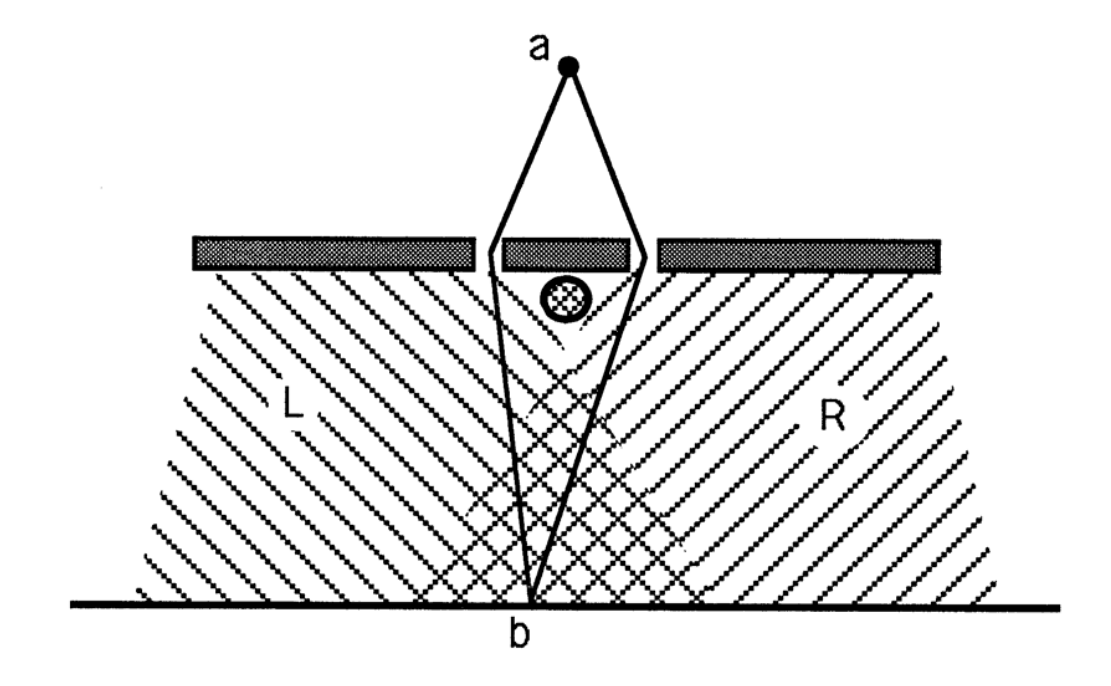
\includegraphics[height=4cm ,width=6.5cm]{QM/AB_effect.png}
	\caption{The Aharonov–Bohm experiment}
\end{figure}\\
Let $\Psi^{(0)}(\bm{x},t)$ be the solution of the Schrödinger equation and boundary conditions of this problem for the case in which the vector potential is everywhere zero. Now let us consider the case in which the magnetic field is non-zero inside the cylinder but zero outside of it. The vector potential $\bm{A}$ will not vanish everywhere in the exterior region, even though $\bm{B}=\bm{\nabla}\times\bm{A}=0$
outside of the cylinder. This follows by applying Stokes's theorem to any path surrounding the cylinder
\[\oint \bm{A}\cdot d\bm{x} = \int\int (\bm{\nabla}\times\bm{A})\cdot d\bm{S} = \int\int \bm{B}\cdot d\bm{S} = \Phi.\]
If the flux through the cylinder is not zero, then the vector potential must be nonzero on every path that encloses the cylinder. However in any simply connected region outside of the cylinder, it is possible to express the vector potential as the gradient of a scalar, from the zero potential solution by means of a gauge transformation, $\Psi = \Psi^{(0)}\exp(ie\Lambda)$.
\\ \\
In region L, which contains the slit on the left, the wave function can be written as $\Psi_{\mathrm{L}} = \Psi_{\mathrm{L}}\exp(ie\Lambda_1)$, where $\Psi_{\mathrm{L}}$ is the zero potential solution in region L, and $\Lambda_1(\bm{x},t) = \int \bm{A}\cdot d\bm{x}$, with the integral taken along a path within region L. A similar form can be written for the wave function in the region R, which contains the slit on the right.
At the point b, in the overlap of regions L and R, the wave function is a superposition of contributions from both slits. Hence we have
\[\Psi(\bm{b}) = \Psi_{\mathrm{L}}\exp(ie\Lambda_1) + \Psi_{\mathrm{R}}\exp(ie\Lambda_2).\]
The interference pattern depends $\exp(ie(\Lambda_1-\Lambda_2)) = \exp(ie\Phi)$. 
Therefore the interference pattern is sensitive to the magnetic flux inside of the cylinder, even though the particles never pass through the region in which the magnetic field is nonzero. 
The AB effect is a topological effect, in that the effect depends on the flux encircled by the paths available to the particle, even though the paths may never approach the region of the flux. 
\\ \\
At last, we conclude that in quantum theory, the potentials themselves are physically significant; however, they are subject to the requirement that all observable effects be invariant under gauge transformations.

\chapter{Angular Momentum}
\section{Eigenvalues of angular momentum operator}
Commutation relations among the angular momentum operators are
\[[J_i,J_j] = \epsilon_{ijk} J_k.\]
And these three operators are self-adjoint. We first introduce the operator $J^2 \equiv J_x^2 + J_y^2 + J_z^2$. We can verify that $[J^2,\bm{J}] = 0$. Thus there exists a complete set of common eigenvectors of $J^2$ and any one component of $\bm{J}$. Particularly, we have the pair of eigenvalue equations
\[J^2 | \beta,m\rangle = \beta | \beta,m\rangle , \quad J_z | \beta,m\rangle = m | \beta,m\rangle.\]
Since
\[\langle \beta,m | J^2 | \beta,m \rangle = \langle \beta,m | J_x^2 | \beta,m \rangle + \langle \beta,m | J_y^2 | \beta,m \rangle + \langle \beta,m | J_z^2 | \beta,m \rangle,\]
we have $m^2 \leq \beta$. Thus for a fixed value of $\beta$ there must be maximum and minimum values for $m$.
Define
\[J_+ \equiv J_x + iJ_y , \quad J_- \equiv J_x - iJ_y.\]
we have commutation relations
\[[J_z,J_+] = J_+ , \quad [J_z,J_-] = -J_- , \quad [J_+,J_-] = 2J_z.\]
Thus
\[J_z J_+ | \beta,m\rangle = J_+(J_z + 1)| \beta,m\rangle = (m+1)J_+| \beta,m\rangle.\]
Therefore, either $J_+ | \beta,m\rangle$ is an eigenvector of $J_z$ with the raised eigenvalue $m+1$, or $J_+ | \beta,m\rangle = 0$. Now for fixed $\beta$ there is a maximum value of $m$, which we shall denote as $j$. It must be the case that
\[J_+ |\beta,j\rangle = 0.\]
Since
\[J_- J_+ = J^2 - J_z^2 - J_z,\]
it is obvious that $\beta = j(j+1)$. By similar method, we can show the minimum eigenvalue of $J_z$ for fixed $\beta$ satisfy that $\beta = k(k-1)$. Therefore, we have $k = -j$.
We have thus shown the existence of a set of eigenvectors corresponding to integer spaced $m$ values in the range $-j \leq m \leq j$. Since the difference between the maximum value $j$ and the minimum value $-j$ must be an integer, it follows that $j = \mbox{ integer} / 2$. Henceforth we shall adopt the common and more convenient notation of labeling the eigenvectors by $j$ instead of by $\beta$. Thus the vector that was previously denoted as $|\beta,m\rangle$ will now be denoted as $|j,m\rangle$. 
\\ \\
To find the matrix element of angular momentum operator, we notice that
\[\langle j,m| J_-J_+|j,m\rangle = j(j+1)-m(m+1).\]
Therefore, we can get
\[J_+ |j,m\rangle = \sqrt{(j+m+1)(j-m)} |j,m+1\rangle.\]
Similarly, we have
\[J_- |j,m\rangle = \sqrt{(j-m+1)(j+m)} |j,m-1\rangle.\]
The matrix element of $J_+$, $J_-$ and $J_z$ are
\[\langle j',m'| J_+ | j,m\rangle = \sqrt{(j+m+1)(j-m)} \delta_{jj'}\delta_{m',m+1}.\]
\[\langle j',m'| J_- | j,m\rangle = \sqrt{(j-m+1)(j+m)} \delta_{jj'}\delta_{m',m-1}.\]
\[\langle j',m'| J_z | j,m\rangle = m \delta_{jj'}\delta_{m',m}.\]

\section{Orbital Angular Momentum and Spin}
Let $\psi(\bm{x})$ be a one-component state function in coordinate representation. When it is subjected to a rotation it is transformed into
\[\bm{R}\psi(\bm{x}) = \psi(R^{-1}\bm{x}),\]
where $\bm{R}$ is the rotation operator generated by $\bm{R} = \exp(-i\bm{J}\cdot\bm{n}\theta)$. For a rotation through infinitesimal angle $\epsilon$ about the $z$ axis, we have
\[\bm{R}_z(\epsilon) \psi(x,y,z) = \psi(x+\epsilon y,y-\epsilon x,z) = \psi(x,y,x) + \epsilon (y \frac{\partial \psi}{\partial x} - x \frac{\partial \psi}{\partial y}).\]
On the other hand, 
\[\bm{R}_z(\epsilon) = I - i\epsilon J_z.\]
Thus we have $J_z = -i(x \frac{\partial}{\partial y} - y \frac{\partial}{\partial x})$. 
This is just the $z$ component of the orbital angular momentum operator $L = \bm{X} \times \bm{P}$.
\\ \\
For a multicomponent state function, we have
\[\bm{R} \left( \begin{matrix} \psi_1(\bm{x}) \\ \psi_2(\bm{x}) \\  \vdots \end{matrix} \right) = D \left( \begin{matrix} \psi_1(R^{-1}\bm{x}) \\ \psi_2(R^{-1}\bm{x}) \\  \vdots \end{matrix} \right).\]
Thus the general form of the rotation operator will be
\[\bm{R}_{n}(\theta) = e^{-i\bm{L}\cdot\bm{n}\theta}D_n(\theta).\]
The two factors commute because the first acts only on the coordinate and the second acts only on the components of the column vector. The matrix $D$ must be unitary, and so it can be written as
\[D_n(\theta) = e^{-i\bm{S}\cdot\bm{n}\theta}.\]
The angular momentum operator $\bm{J}$ has the form
\[\bm{J} = \bm{L} + \bm{S}\]
with $\bm{L} = \bm{X} \times \bm{P}$ and $[L_{\alpha},S_{\beta}] = 0$. In the particular representation used in this section, we have $\bm{L} = -i\bm{x}\times\bm{\nabla}$, and the components of $S$ are
discrete matrices. The operators $\bm{L}$ and $\bm{S}$ are called the orbital and spin parts of the angular momentum.

\subsubsection{Orbital angular momentum}
The form of the gradient operator in spherical coordinates is
\[\bm{\nabla} = \bm{e}_r \frac{\partial}{\partial r} + \bm{e}_{\theta} \frac{1}{r} \frac{\partial}{\partial \theta} + \bm{e}_{\phi} \frac{1}{r\sin\theta} \frac{\partial}{\partial \phi}.\]
The orbital angular momentum operator then has the form
\[\bm{L} = r\bm{e}_r \times (-i\bm{\nabla}) = (-i) \left[ \bm{e}_{\phi} \frac{\partial}{\partial \theta} - \bm{e}_{\theta} \frac{1}{\sin\theta} \frac{\partial}{\partial \phi} \right].\]
Therefore, we have
\[L_z = \bm{L}\cdot\bm{e}_z = -i\frac{\partial}{\partial \phi},\]
\[L^2 = \bm{L}\cdot\bm{L} = - \left [ \frac{1}{\sin\theta} \frac{\partial }{\partial \theta} (\sin\theta \frac{\partial }{\partial \theta}) + \frac{1}{\sin^2\theta} \frac{\partial^2}{\partial \phi^2}  \right ].\]
We must now solve the two coupled differential equations,
\[L_z Y(\theta,\phi) = m Y(\theta,\phi) , \quad L^2 Y(\theta,\phi) = l(l+1) Y(\theta,\phi).\]
Apart from normalization, we have $Y(\theta,\phi) = e^{im\phi}P_l^m(\cos\theta)$. Here, $P_l^m$ is the \href{https://en.wikipedia.org/wiki/Associated_Legendre_polynomials}{associated Legendre polynomials}. If we assume that the solution must be single-valued under rotation, then it will follow that $m$ must be an integer. If we further assume that it must be nonsingular at $\theta = 0$ and $\theta = \pi$, then from the standard theory of the Legendre equation it will follow that $l$ must be a nonnegative integer in the range $l \geq |m|$. The normalized solutions that result from these assumptions are the well-known \href{https://en.wikipedia.org/wiki/Spherical_harmonics}{spherical harmonics}
\[Y_l^m(\theta,\phi) = (-1)^{(m+|m|)/2} \left [\frac{(2l+1)(l-|m|)!}{4\pi(l+|m|)!}  \right ]^{1/2}e^{im\phi} P_l^{|m|}(\cos\theta).\]

\subsubsection{Spin}
A particular species of particle is characterized by a set of quantum numbers that includes the value of its spin $s$, it is often sufficient to treat the spin operators $\bm{S}$ as acting on the space of dimension
$2s+1$ that is spanned by the eigenvectors of for a fixed value of $s$. 
\\ \\
If $s= \frac{1}{2}$, we have
\[S_x = \frac{1}{2} \left[ \begin{matrix} 0& 1\\ 1& 0\end{matrix} \right] , \quad S_y = \frac{1}{2} \left[ \begin{matrix} 0& -i\\ i& 0\end{matrix} \right] , \quad S_z = \frac{1}{2} \left[ \begin{matrix} 1& 0\\ 0& -1\end{matrix} \right].\]
The spin operator in direction $\bm{n} = (\sin\theta\cos\phi,\sin\theta\sin\phi,\cos\theta)$ is
\[\bm{S}_{n} = \frac{1}{2} \left[ \begin{matrix} \cos\theta& e^{-i\phi}\sin\theta\\ e^{i\phi}\sin\theta& -\cos\theta\end{matrix} \right].\]
The eigenvectors are
\[\left[ \begin{matrix} e^{-i\phi/2}\cos\frac{\theta}{2}\\ e^{i\phi/2}\sin\frac{\theta}{2} \end{matrix} \right] , \quad \left[ \begin{matrix} -e^{-i\phi/2}\sin\frac{\theta}{2}\\ e^{i\phi/2}\cos\frac{\theta}{2} \end{matrix} \right],\]
corresponding to eigenvalues $\frac{1}{2}$ and $-\frac{1}{2}$.
\\ \\
If $s= 1$, we have
\[S_x = \sqrt{\frac{1}{2}} \left[ \begin{matrix} 0& 1& 0\\ 1& 0& 1\\ 0& 1& 0\end{matrix} \right]  , \quad S_y = \sqrt{\frac{1}{2}} \left[ \begin{matrix} 0& -i& 0\\ i& 0& -i\\ 0& i& 0\end{matrix} \right] , \quad S_z = \sqrt{\frac{1}{2}} \left[ \begin{matrix} 1& 0& 0\\ 0& 0& 0\\ 0& 0& -1\end{matrix} \right].\]
The spin operator in direction $\bm{n} = (\sin\theta\cos\phi,\sin\theta\sin\phi,\cos\theta)$ is
\[\bm{S}_{n} =  \left[ \begin{matrix} \cos\theta& \sin\theta e^{-i\phi} \sqrt{\frac{1}{2}}& 0\\ \sin\theta e^{i\phi}\sqrt{\frac{1}{2}}& 0& \sin\theta e^{-i\phi} \sqrt{\frac{1}{2}}\\ 0& \sin\theta e^{i\phi} \sqrt{\frac{1}{2}}& -\cos\theta\end{matrix} \right].\]
The eigenvectors are
\[\left[ \begin{matrix} \frac{1}{2}(1+\cos\theta)e^{-i\phi}\\ \sqrt{\frac{1}{2}}\sin\theta \\ \frac{1}{2}(1-\cos\theta)e^{i\phi} \end{matrix} \right] , \quad \left[ \begin{matrix} -\sqrt{\frac{1}{2}}\sin\theta e^{-i\phi}\\ \cos\theta \\ \sqrt{\frac{1}{2}}\sin\theta e^{i\phi} \end{matrix} \right] , \quad \left[ \begin{matrix} \frac{1}{2}(1-\cos\theta)e^{-i\phi}\\ -\sqrt{\frac{1}{2}}\sin\theta \\ \frac{1}{2}(1+\cos\theta)e^{i\phi} \end{matrix} \right],\]
corresponding to eigenvalues $1$, $0$ and $-1$.

\section{Rotation operator}
Three parameters are required to describe an arbitrary rotation. A common parameterization is by the Euler angles. From the fixed system of axes $Oxyz$, a new rotated set of axes $Ox'y'z'$ is produced in three steps:
\begin{itemize}
\item Rotate through angle $\alpha$ about $Oz$, carrying $Oy$ into $Ou$.
\item Rotate through angle $\beta$ about $Ou$, carrying $Oz$ into $Oz'$.
\item Rotate through angle $\gamma$ about $Oz'$ , carrying $Ou$ into $Oy'$.
\end{itemize}
\begin{figure}[!h]
	\centering
	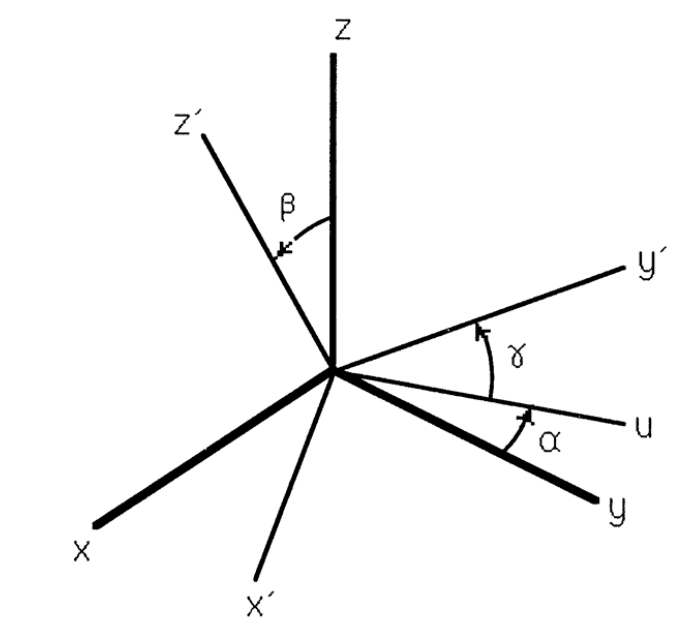
\includegraphics[height=4.5cm ,width=5cm]{QM/rotation.png}
	\caption{Euler angles}
\end{figure}
The net rotation is
\[\bm{R}(\alpha,\beta,\gamma) = \bm{R}_{z'}(\gamma) \bm{R}_{u}(\beta) \bm{R}_{z}(\alpha) = e^{-i\gamma J_{z'}} e^{-i\beta J_{u}} e^{-i\alpha J_{z}}.\]
Since $J_u = \bm{R}_z(\alpha) J_y \bm{R}_z(-\alpha)$, we have $\bm{R}_u(\beta) = \bm{R}_z(\alpha) \bm{R}_y(\beta) \bm{R}_z(-\alpha)$. Similarly, we can obtain $\bm{R}_{z'}(\gamma) = \bm{R}_{u}(\beta) \bm{R}_z(\gamma) \bm{R}_u(-\beta)$. Therefore, the rotation operator is
\[\bm{R}(\alpha,\beta,\gamma) = \bm{R}_{z}(\alpha) \bm{R}_{y}(\beta) \bm{R}_{z}(\gamma) = e^{-i\alpha J_{z}} e^{-i\beta J_{y}} e^{-i\gamma J_{z}}.\]
The matrix representation of the rotation operator in the basis $|j,m\rangle$
\[\langle j',m' | \bm{R}(\alpha,\beta,\gamma) | j,m \rangle = \delta_{jj'} D_{m'm}^{(j)}(\alpha,\beta,\gamma)\]
gives rise to the rotation matrices,
\[D_{m'm}^{(j)}(\alpha,\beta,\gamma) \equiv \langle j,m' | e^{-i\alpha J_{z}} e^{-i\beta J_{y}} e^{-i\gamma J_{z}} | j,m \rangle = e^{-i(\alpha m' + \gamma m)} d_{mm'}^{(j)}(\beta),\]
where
\[ d_{m'm}^{(j)}(\beta) \equiv \langle j,m' | e^{-i\beta J_{y}} | j,m \rangle.\]
For the case of $j = \frac{1}{2}$, we have $J_y = \frac{1}{2}\sigma_y$ and $\sigma_y^2 = I$. We can obtain
\[d^{(1/2)}(\beta) = \left[ \begin{matrix} \cos \frac{\beta}{2} & -\sin \frac{\beta}{2} \\ \cos \frac{\beta}{2}& \sin \frac{\beta}{2}\end{matrix} \right] .\]
Notice that this matrix is periodic in $\beta$ with period $4\pi$, but it changes sign when $2\pi$ is added to $\beta$. This double-valuedness under rotation by $2\pi$ is a characteristic of the full rotation matrix whenever $j$ is a half odd-integer. The matrix is single-valued under rotation by $2\pi$ whenever $j$ is an integer.
\\ \\
Rotation of angular momentum eigenvectors now can be written as
\[\bm{R}(\alpha,\beta,\gamma)|j,m\rangle = \sum_{m'} D_{m'm}^{(j)}(\alpha,\beta,\gamma) |j,m'\rangle.\]
When it comes to spherical harmonics, we have
\[Y_l^m(\theta',\phi') = \bm{R}^{-1}((\alpha,\beta,\gamma)) Y_l^m(\theta,\phi) = \sum_{m'} Y_{l}^{m'}(\theta,\phi) [D_{mm'}^{(j)}((\alpha,\beta,\gamma))]^*.\]
By putting $\beta = \gamma = 0$ we obtain
\[Y_l^m(\theta,\phi+\alpha) = \sum_{m'} Y_{l}^{m'}(\theta,\phi) [D_{mm'}^{(j)}((\alpha,0,0))]^* = e^{i\alpha m} Y_{l}^{m}(\theta,\phi).\]
Setting $\phi=0$ then yields
\[Y_l^m(\theta,\alpha) = e^{i\alpha m} Y_{l}^{m}(\theta,0).\]
Since the direction $\theta = 0$ is the polar axis, continuity of the spherical harmonic requires that $Y_l^m(0,\alpha)$ be independent of $\alpha$. Therefore we must
have $Y_l^m(0,0) = 0$ for $m \neq 0$, and so we can write
\[Y_{l}^{m}(0,0) = c_{l}\delta{m0}.\]
Then we have
\[Y_l^m(\theta,\phi) = \sum_{m'} Y_{l}^{m'}(0,0) [D_{mm'}^{(j)}((\phi,\theta,\gamma))]^* = c_l [D_{m0}^{(j)}((\phi,\theta,\gamma))]^*\]
for arbitrary $\gamma$, thus obtaining a simple relation between the spherical harmonics and the rotation matrices. Conventional normalization is obtained if we put
\[c_l = \left( \frac{2l+1}{4\pi} \right) ^{1/2}.\]
The operator for a rotation through $2\pi$ about an axis
along the unit vector $\bm{n}$ is $\bm{R}_n(2\pi) = e^{-2\pi i\bm{n}\cdot\bm{J}}$. Its effect on the standard angular momentum eigenvectors is
\[\bm{R}_n(2\pi) = (-1)^{2j}|j,m\rangle .\]
We assume a rotation through $2\pi$ as a trivial operation that leaves everything unchanged, i.e. all dynamical variables are invariant under $2\pi$ rotation:
\[\bm{R}(2\pi) A \bm{R}^{-1}(2\pi) = A,\]
where $A$ may represent any physical observable. 
\\ \\
The operator $\bm{R}_{2\pi}$ divides the vector space into two subspaces. A typical vector in the first subspace,
denoted as $|+\rangle$, has the property $\bm{R}(2\pi)|+\rangle = |+\rangle$, whereas a typical vector in the second subspace, denoted as $|-\rangle$, has the property $\bm{R}(2\pi)|-\rangle = -|-\rangle$. Now, if $A$ represents any physical observable, we have $\langle + | \bm{R}(2\pi) A| - \rangle = \langle + | A\bm{R}(2\pi)| - \rangle$, leading to 
\[\langle + | A | - \rangle = 0.\]
No physical observable can have nonvanishing matrix elements between states with integer angular momentum and states with half odd-integer angular momentum. This fact forms the basis of a superselection rule: There is no observable distinction among the state vectors of the form
\[|\Psi_{\omega}\rangle = |+\rangle + e^{i\omega}|-\rangle\]
for different values of the phase $\omega$.

\section{Addition of angular momentum}
Let us consider a two-component system, each component of which has angular momentum degrees of freedom. Basis vectors for the composite system can be formed from the basis vectors of the components by taking all binary products of a vector from each set
\[|j_1,j_2,m_1,m_2\rangle = |j_1,m_1\rangle ^{(1)} |j_2,m_2\rangle ^{(2)}.\]
These vectors are common eigenvectors of the four commutative operators $\bm{J}^{(1)}\cdot\bm{J}^{(1)}$, $\bm{J}^{(2)}\cdot\bm{J}^{(2)}$, $\bm{J}_z^{(1)}$, and $\bm{J}_z^{(2)}$.
It is often desirable to form eigenvectors of the total angular momentum operators, $\bm{J}\cdot\bm{J}$ and $\bm{J}_z$, where the total angular momentum vector operator is
\[\bm{J} = \bm{J}^{(1)}\otimes\bm{1} + \bm{1}\otimes\bm{J}^{(2)}.\]
This is useful when the system is invariant under rotation as a whole, but not under rotation of the two components separately. 
The eigenvectors of $\bm{J}\cdot\bm{J}$ and $\bm{J}_z$ may be denoted as $|\alpha, J, M \rangle$. It is easy to verify that the four operators $\bm{J}^{(1)}\cdot\bm{J}^{(1)}$, $\bm{J}^{(2)}\cdot\bm{J}^{(2)}$, $\bm{J}\cdot\bm{J}$ and $\bm{J}_z$ are mutually commutative, and hence they possess a complete set of common eigenvectors. 
Since the set of product vectors and the new set of total angular momentum eigenvectors are both eigenvectors of $\bm{J}^{(1)}\cdot\bm{J}^{(1)}$ and $\bm{J}^{(2)}\cdot\bm{J}^{(2)}$, the eigenvalues $j_1$ and $j_2$ will be constant in both sets. Therefore
we may confine our attention to the vector space of dimension $(2j_1+1)(2j_2+1)$ that is spanned by product vectors with fixed values of $j_1$ and $j_2$.
\\ \\
Now the $2J+1$ vectors $|\alpha, J, M \rangle$, with $M$ in the range $-J \leq M \leq J$, span an irreducible subspace.
Therefore if the vector $|\alpha, J, M \rangle$, for a particular value of $M$, can be constructed in the space under consideration, then so can the entire set of $2J+1$
such vectors with $M$ in the range $-J \leq M \leq J$.
For a particular value of $J$, it might be possible to construct one such set of vectors, two or more linearly independent sets, or none at all.
Let $N(J)$ denotes the number of independent sets that can be constructed. Let $n(M)$ be the degree of degeneracy, in this space, of the eigenvalue $M$ . The relation between these two quantities is
\[n(M) = \sum_{J \geq |M|} N(J),\]
and hence
\[N(J) = n(J) - n(J+1).\]
The product vectors $|j_1,m_1\rangle |j_2,m_2\rangle$ are eigenvectors of the operator $\bm{J}_z$, with eigenvalue $m_1+m_2$, and the degree of degeneracy $n(M)$ is equal to the number of pairs $(m_1,m_2)$ such that $M=m_1+m_2$.
\begin{figure}[!h]
	\centering
	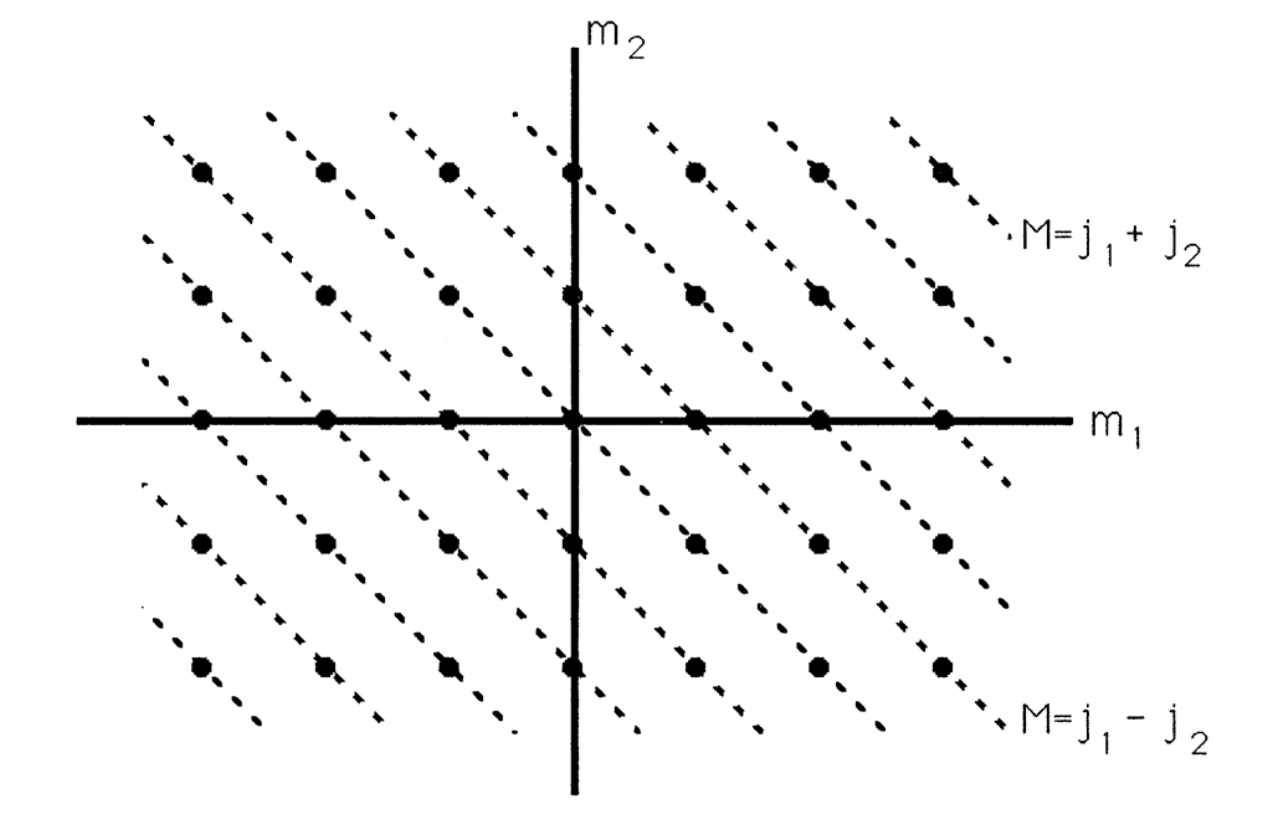
\includegraphics[height=4.14cm ,width=6.4cm]{QM/angular_momentum.png}
	\caption{Possible values of $M=m_1+m_2$ , illustrated for $j_1=3$, $j_2=2$}
\end{figure}
Therefore,
\[n(M)=\begin{cases} 0 , \quad |M| > j_1 + j_2\\ j_1+j_2+1-|M|, \quad |j_1-j_2| \leq M \leq |j_1+j_2|\\ 2j_{\mathrm{min}}+1 , \quad 0 \leq |M|\leq |j_1-j_2|\end{cases} .\]
It then follows that
\[N(J)=\begin{cases} 1 , \quad |j_1-j_2| \leq J \leq |j_1+j_2|\\ 0 , \quad \mbox{otherwise}\end{cases} .\]
It has turned out that $N(J)$ is never greater that $1$, and so the vectors $|\alpha, J, M \rangle$ can be uniquely labelled by the eigenvalues of the four operators $\bm{J}^{(1)}\cdot\bm{J}^{(1)}$, $\bm{J}^{(2)}\cdot\bm{J}^{(2)}$, $\bm{J}\cdot\bm{J}$ and $\bm{J}_z$. Henceforth these total angular momentum
eigenvectors will be denoted as $|j_1,j_2,J,M\rangle$. And we have the unitarity transformation 
\[|j_1,j_2,J,M\rangle = \sum_{m_1,m_2} |j_1,j_2,m_1,m_2\rangle \langle j_1,j_2,m_1,m_2 | j_1,j_2,J,M\rangle.\]
The coefficients of this transformation are called the Clebsch–Gordan coefficients, denoted as $(j_1,j_2,m_1,m_2|J,M)$.
The phases of the CG coefficients are not yet defined because of the indeterminacy of the relative phases of the vectors $|j_1,j_2,J,M\rangle$. For different values of $M$ but fixed $J$ we adopt the usual phase convention that led to
\[J_+ |j_1,j_2,J,M\rangle = \sqrt{(J+M+1)(J-M)} |j_1,j_2,J,M+1\rangle.\]
This leaves one arbitrary phase for each $J$ value, which we fix by requiring that $(j_1,j_2,j_1,J-j_1|J,J)$ be real and positive. It can be shown that all of the CG coefficients are now real.
We can also prove that CG coefficients vanishe unless following conditions are satisfied:
\begin{itemize}
\item $m_1+m_2=M$.
\item $|j_1-j_2| \leq J \leq |j_1+j_2|$.
\item $j_1+j_2+J =$ an integer.
\end{itemize}
It is possible to work out the values of the CG coefficients by successive application of the raising or lowering operator to
\[|j_1,j_2,J,M\rangle = \sum_{m_1,m_2} |j_1,j_2,m_1,m_2\rangle (j_1,j_2,m_1,m_2|J,M).\]
The details of the calculation can be found in section 7.7 of \emph{Quantum mechanics - a modern development(Leslie E. Ballentine)}.And we have \href{https://en.wikipedia.org/wiki/Table_of_Clebsch-Gordan_coefficients}{Table of CG coefficients} and \href{http://www.wolframalpha.com/input/?i=CG+coefficient}{Calculator of CG coefficients} on the internet. A special case of angular momentum addition is spin–orbit coupling of spin $\frac{1}{2}$ particles, and we list the corresponding CG coefficients $(l,\frac{1}{2}, M-m_s, m_s|J,M)$ in the table 17.1.
\begin{table}[!th]
\centering
\begin{tabular}{|c|c|c|}
\hline
 & $J=l+\frac{1}{2}$ & $J=l-\frac{1}{2}$ \\
 \hline
 $m_s = \frac{1}{2}$ & $\left[ \frac{l+M+\frac{1}{2}}{2l+1}\right ]^{\frac{1}{2}} $ & $-\left[ \frac{l-M+\frac{1}{2}}{2l+1}\right ]^{\frac{1}{2}} $ \\
 \hline
 $m_s = -\frac{1}{2}$ & $\left[ \frac{l-M+\frac{1}{2}}{2l+1}\right ]^{\frac{1}{2}} $ & $\left[ \frac{l+M+\frac{1}{2}}{2l+1}\right ]^{\frac{1}{2}} $ \\
\hline
\end{tabular}
\caption{Spin-Orbit coupling}
\end{table}\\
Now let us consider the relation between CG coefficients and rotation matrices. On the one hand, we have
\[\langle j_1,j_2,m_1,m_2 | \bm{R} | j_1,j_2,m'_1,m'_2\rangle = D_{m_1m'_1}^{(j_1)}(R) D_{m_2m'_2}^{(j_2)}(R).\]
On the other hand, we have
\begin{eqnarray}
&\phantom{=}& \langle j_1,j_2,m_1,m_2 | \bm{R} | j_1,j_2,m'_1,m'_2\rangle \nonumber \\
&=& \sum_{J,M,J',M'} (j_1,j_2,m_1,m_2|J,M) (j_1,j_2,m'_1,m'_2|J',M')  \langle j_1,j_2,J,M | \bm{R} | j_1,j_2,J',M'\rangle \nonumber \\
&=& \sum_{J,M,M'} (j_1,j_2,m_1,m_2|J,M) (j_1,j_2,m'_1,m'_2|J,M')D_{MM'}^{(J)}(R) .\nonumber
\end{eqnarray}
Therefore, we can get
\[D_{m_1m'_1}^{(j_1)}(R) D_{m_2m'_2}^{(j_2)}(R) = \sum_{J,M,M'} (j_1,j_2,m_1,m_2|J,M) (j_1,j_2,m'_1,m'_2|J,M')D_{MM'}^{(J)}(R).\]
It is called Clebsch-Gordan series.
\\ \\
Recall that
\[Y_l^m(\theta,\phi) =  \left( \frac{2l+1}{4\pi} \right) ^{1/2} [D_{m0}^{(j)}((\phi,\theta,0))]^* .\]
Thus we have
\[Y_{l_1}^{m_1}(\theta,\phi) Y_{l_2}^{m_2}(\theta,\phi) = \sum_{l,m} \sqrt{\frac{(2l_1+1)(2l_2+1)}{4\pi(2l+1)}} (l_1,l_2,m_1,m_2|l,m) (l_1,l_2,0,0|l,0) Y_l^m(\theta,\phi).\]
The orthogonal relation of spherical harmonics then would imply that
\[\int d\Omega Y_l^{m*}(\theta,\phi)Y_{l_1}^{m_1}(\theta,\phi) Y_{l_2}^{m_2}(\theta,\phi) = \sqrt{\frac{(2l_1+1)(2l_2+1)}{4\pi(2l+1)}} (l_1,l_2,m_1,m_2|l,m) (l_1,l_2,0,0|l,0).\]

\section{Tensor operators}
Suppose the state of the system is $|\psi\rangle$, then the state after rotation $R$ is $U(R)|\psi\rangle$, denoted as $|\psi'\rangle$. An operator $K$ is called scalar operator if and only if
\[\langle \psi' | K | \psi' \rangle = \langle \psi | K | \psi\rangle,\]
i.e.
\[U^{-1}(R)KU(R) = K.\]
Taking the case of infinitesimal rotation, we can derive that
\[[\bm{J},K] = 0.\]
A group of operators $\bm{V}$ is called vector operator if and only if
\[\langle \psi' | V_i | \psi' \rangle = R_{ii'} \langle \psi | V_{i'} | \psi\rangle,\]
i.e.
\[U^{-1}(R)V_{i}U(R) = \sum_{i'} R_{ii'} V_{i'}.\]
Taking the case of infinitesimal rotation, we can derive that
\[[J_i, V_j] = i\epsilon_{ijk}V_k.\]
If $\bm{V}$ and $\bm{W}$ are vector operators, we can prove that $\bm{V} \cdot \bm{W}$ is scalar operator and $\bm{V} \times \bm{W}$ is vector operator.
\\ \\
Similarly, tensor operators are defined as
\[U^{-1}(R) T_{ij\cdots k} U(R) = \sum_{i'\cdots} R_{ii'} R_{jj'} \cdots R_{kk'} T_{i'j'\cdots k'}.\]
Such a tensor is known as a Cartesian tensor.
The trouble with a Cartesian tensor is that it is reducible, i.e. it can be decomposed into objects that transform independently under rotations. For example, the trace of a tensor transform like a scalar under rotations. 
Thus we now define spherical tensor operators which are irreducible under rotations.  We define a spherical tensor operator of rank $k$ with $(2k+1)$ components as
\[U^{-1}(R) T^{(k)}_q U(R) = \sum_{q'=-k}^{k} [D^{(k)}_{qq'}(R)]^* T^{(k)}_{q'},\]
or equivalently
\[U(R) T^{(k)}_q U^{-1}(R) = \sum_{q'=-k}^{k} D^{(k)}_{q'q}(R) T^{(k)}_{q'},\]
where $D^{(k)}_{qq'}$ is the rotation matrix.
Taking the case of infinitesimal rotation, we can derive that
\[[J_{\pm},T^{(k)}_{q}] = \sqrt{(k \mp q)(k \pm q +1)} T^{(k)}_{q \pm 1},\]
\[[J_z, T^{(k)}_{q}] = q T^{(k)}_{q}.\]
For example, spherical components of a vector operator $\bm{V}$, 
\[V_{-1} = \frac{V_x - i V_y}{\sqrt{2}} , \quad V_0 = V_z , \quad V_{1} = -\frac{V_x + i V_y}{\sqrt{2}} ,\]
satisfy the commutation relation above, so they are spherical tensor of rank $1$. Generally, if $\bm{V}$ is a vector operator, then $Y_l^m(\bm{V})$ is a spherical tensor of ranks $l$.
\\ \\
Spherical tensors can be formed as products of other spherical  tensors, we have following theorem:
\\

\begin{newthem}
Let $X^{(k_1)}_{q_1}$ and $Z^{(k_2)}_{q_2}$ be irreducible spherical tensors of rank $k_1$ and $k_2$. Then
\[T^{(k)}_{q} = \sum_{q_1,q_2} (k_1,k_2,q_1,q_2|k,q) X^{(k_1)}_{q_1} Z^{(k_2)}_{q_2}\]
is an irreducible spherical tensor of rank $k$. 
\end{newthem}
\noindent
The proof can be found in section 3.10 of \emph{Modern Quantum Mechanics(J.J.Sakurai)}.

\begin{example}
suppose $\bm{V}$ and $\bm{U}$ are spherical tensor of rank $1$, then
\[T^{(0)}_{0} = \sqrt{\frac{1}{3}} (U_{-1}V_{1} + U_{1}V_{-1}-U_{0}U_{0}) = - \sqrt{\frac{1}{3}} (U_xV_x + U_yV_y + U_zV_z).\]
is a spherical tensor of rank $0$.
\end{example}

\noindent
Another important theorem on tensor operator is Wigner-Eckart theorem:\\

\begin{newthem}[Wigner-Eckart theorem]
The matrix elements of tensor operators with respect to angular-momentum eigenstates satisfy
\[\langle \tau',j',m'| T^{(k)}_{q}| \tau,j,m\rangle = (j,k,m,q|j',m') \frac{\langle \tau',j' || T^{(k)} || \tau,j\rangle}{\sqrt{2j+1}}.\]
where the double-bar matrix element is independent of $m$ and $m'$ and $q$.
\end{newthem}

\noindent
The proof can be found in section 3.10 of \emph{Modern Quantum Mechanics(J.J.Sakurai)}.
Therefore, for scaler operator $K$, we have
\[\langle \tau',j',m'| S| \tau,j,m\rangle = \delta_{jj'}\delta_{mm'} \frac{\langle \tau',j' || S || \tau,j\rangle}{\sqrt{2j+1}}.\]
For spherical tensor of rank $1$, we have
\[\langle \tau',j',m'| V_{q} | \tau,j,m\rangle = (j,1,m,q|j',m') \frac{\langle \tau',j' || V_q || \tau,j\rangle}{\sqrt{2j+1}}.\]
It would vanish unless
\[m'-m = q , \quad j'-j = 0,1,-1 , \quad j \mbox{ and } j' \mbox{ are not both  } 0.\]
For $j=j'$, Wigner-Eckart theorem - when applied to the vector operator- takes a particularly simple form. We can derive that
\[\langle \tau',j,m' | V_q | \tau, j ,m \rangle = \frac{\langle \tau',j,m | \bm{J}\cdot\bm{V} | \tau, j ,m \rangle}{j(j+1)} \langle j,m' | J_q | j ,m \rangle.\]

\begin{example}
The magnetic moment operator for an atom has the form
\[\bm{\mu} = \frac{-e}{2m_{\mathrm{e}} } (g_{\mathrm{L}}\bm{L} + g_{\mathrm{S}} \bm{S}).\]
The parameters $g_{\mathrm{L}}$ and $g_{\mathrm{S}}$ have approximately the
values $g_{\mathrm{L}} = 1$ and $g_{\mathrm{S}} = 2$. The former is an generalization of the magnetic moment we worked out in classical electrodynamics for a system of charged particles. The latter will be discussed in quantum field theory.
We define the effective Lande factor as
\[\langle \tau,J,M' | \bm{\mu} | \tau,J,M \rangle = \frac{-e}{2m_{\mathrm{e}} } g_{\mathrm{eff}} \langle J,M' | \bm{J} | J,M \rangle.\]
Then, we have
\[g_{\mathrm{eff}} = \frac{\langle \tau,J,M | g_{\mathrm{L}}\bm{L}\cdot\bm{J} + g_s \bm{S}\cdot\bm{J} | \tau,J,M \rangle}{J(J+1)} = 1 + \frac{J(J+1)- L(L+1) + S(S+1)}{2J(J+1)}.\]
\end{example}

\section{Spherical potential well}
The stationary states of a particle in the spherical potential well are determined by
\[-\frac{1}{2m}\nabla^2 \Psi  + W(r) \Psi = E\Psi .\]
In spherical coordinates, 
\[\nabla^2 = \frac{1}{r^2} \frac{\partial}{\partial r} \left [ r^2\frac{\partial}{\partial r} \right ] + \frac{1}{r^2\sin\theta} \frac{\partial}{\partial \theta} \left [\sin\theta \frac{\partial}{\partial \theta} \right ] + \frac{1}{r^2\sin^2\theta} \frac{\partial^2}{\partial\phi^2}.\]
Therefore, the eigenvalue equation becomes
\[-\frac{1}{2m} \frac{1}{r^2} \frac{\partial}{\partial r} \left [ r^2\frac{\partial \Psi}{\partial r}\right ]  + \frac{L^2}{2Mr^2} \Psi + W(r)\Psi = E\Psi.\]
Suppose the eigenfunctions have the factored form
\[\Psi(r,\theta,\phi) = Y_l^m(\theta,\phi) \frac{u(r)}{r}.\]
The radial function then satisfies the equation
\[-\frac{1}{2m} \frac{d^2 u(r)}{dr^2} + \left[ \frac{l(l+1)}{2mr^2} + W(r)\right]u(r) = Eu(r).\]
The radial function must satisfy the boundary condition $u(0) = 0$ since $\Psi(r,\theta,\phi)$ would otherwise have an $r^{-1}$ singularity at the origin. The normalization $\langle \Psi | \Psi \rangle = 1$ implies that
\[\int_0^{\infty} = |u(r)|^2 dr = 1.\]

\subsubsection{The hydrogen atom}
The hydrogen atom is a two-particle system consisting of an electron and a proton. The Hamiltonian is
\[H = \frac{P_{\mathrm{e}}^2}{2m_{\mathrm{e}}} + \frac{P_{\mathrm{p}}^2}{2m_{\mathrm{p}}} - \frac{e^2}{4\pi|\bm{Q}_{\mathrm{e}}-\bm{Q}_{\mathrm{p}}|}.\]
We take as independent variables the center of mass and relative coordinates of the particles
\[\bm{Q}_{\mathrm{c}} = \frac{m_{\mathrm{e}}\bm{Q}_{\mathrm{e}} + m_{\mathrm{p}}\bm{Q}_{\mathrm{p}}}{m_{\mathrm{e}}+m_{\mathrm{p}}} , \quad \bm{Q}_{\mathrm{r}} = \bm{Q}_{\mathrm{e}}-\bm{Q}_{\mathrm{p}}.\]
The corresponding momentum operators are
\[\bm{P}_{\mathrm{c}} = \bm{P}_{\mathrm{e}} + \bm{P}_{\mathrm{p}} , \quad \bm{P}_{\mathrm{r}} = \frac{m_{\mathrm{p}}\bm{P}_{\mathrm{e}}-m_{\mathrm{e}}\bm{P}_{\mathrm{p}}}{m_{\mathrm{e}} + m_{\mathrm{p}}}.\]
We can verify that
\[[Q_{\mathrm{c}\alpha},P_{\mathrm{c}\beta}] = [Q_{\mathrm{r}\alpha},P_{\mathrm{r}\beta}] = i\delta_{\alpha\beta} , \quad [Q_{\mathrm{c}\alpha},P_{\mathrm{r}\beta}] = [Q_{\mathrm{r}\alpha},P_{\mathrm{c}\beta}] = 0.\]
The Hamiltonian becomes
\[H = \frac{P_{\mathrm{c}}^2}{2(m_{\mathrm{e}}+m_{\mathrm{p}})} + \frac{P_{\mathrm{r}}^2}{2\mu} - \frac{e^2}{4\pi|\bm{Q}_{\mathrm{r}}|},\]
where $\mu$ is called the reduced mass, and is defined by $\mu \equiv \frac{m_{\mathrm{e}}m_{\mathrm{p}}}{m_{\mathrm{e}}+m_{\mathrm{p}}}$.
The center of mass behaves as a free particle, and its
motion is not coupled to the relative coordinate. We shall confine our attention to the internal degrees of freedom described by the relative coordinate $\bm{Q}_{\mathrm{r}}$. The energy eigenvalue equation in coordinate representation is
\[-\frac{1}{2\mu}\nabla^2 \Psi(\bm{r})  -\frac{e^2}{4\pi r} \Psi(\bm{r}) = E\Psi(\bm{r}).\]
Suppose $\Psi(r,\theta,\phi) = Y_l^m(\theta,\phi) \frac{u(r)}{r}$, we have
\[-\frac{1}{2\mu} \frac{d^2 u(r)}{dr^2} + \left[ \frac{l(l+1)}{2\mu r^2} - \frac{e^2}{4\pi r}\right]u(r) = Eu(r).\]
Define
\[\rho \equiv \alpha r , \quad \alpha \equiv \sqrt{8\mu|E|} , \quad \lambda \equiv \frac{e^2}{4\pi} \sqrt{\frac{\mu}{2|E|}}.\]
We have
\[\frac{d^2 u}{d\rho^2} + \left[ -\frac{1}{4} + \frac{\lambda}{\rho} - \frac{l(l+1)}{\rho^2} \right] u = 0.\]
As $\rho \to \infty$, we have $u \sim e^{-\rho/2}$. And as $\rho \to 0$, we have $u \sim \rho^{l+1}$. Therefore, we can suppose
\[u(\rho) = \rho^{l+1} e^{-\rho/2} v(\rho).\]
And we can get
\[\rho \frac{d^2 v}{d\rho^2} + (2l+2-\rho)\frac{dv}{d\rho} + (\lambda-l-1)v = 0.\]
It is the so-called \href{http://mathworld.wolfram.com/ConfluentHypergeometricDifferentialEquation.html}{Confluent Hypergeometric Differential Equation}.
When $\lambda - 1- l = n_r$, we have regular solutions. Solutions are \href{https://en.wikipedia.org/wiki/Laguerre_polynomials#Generalized_Laguerre_polynomials}{Associated Laguerre Polynomial}, and will be denoted as $L_{n-l-1}^{2l+1}(\rho) (n=n_r+l+1)$. The energy levels are
\[E_n = -\frac{\mu e^4}{32\pi^2 n^2}.\]
The degeneracy of an eigenvalue $E_n$ is
\[\sum_{l=0}^{n-1} (2l+1) = n^2.\]
\begin{note}
The degeneracy of an energy level of a hydrogen atom is greater than this by a factor of $4$, which arises from the two-fold orientational degeneracies of the electron and proton spin states. This four-fold degeneracy is modified by the hyperfine interaction between the magnetic moments of the electron and the proton.
\end{note}
\noindent
The orthonormal energy eigenfunctions for the hydrogen atom are
\[\Psi_{nlm}(r,\theta,\phi) =  \left[ \frac{4(n-l-1)!}{(na_0)^3 n[(n+l)!]^3} \right]^{\frac{1}{2}} \rho^l L_{n-l-1}^{2l+1}(\rho) e^{-\rho/2} Y_l^m (\theta,\phi),\]
where $\rho = \alpha r = {2r}/{na_0}$, and $a_0 \equiv {4\pi}/{\mu e^2}$ is a characteristic length for the
atom, known as the Bohr radius.The ground state wave
function is
\[\Psi_{000} = (\pi a_0^3)^{-\frac{1}{2}} e^{-\frac{r}{a_0}}.\]
A measure of the spatial extent of the bound states of hydrogen is given by the averages of various powers of the distance $r$:
\begin{eqnarray}
\langle r \rangle &=& n^2a_0 \left \{ 1 + \frac{1}{2} \left [ 1 - \frac{l(l+1)}{n^2} \right] \right\} ,\nonumber \\
\langle r^2 \rangle &=& n^4a_0^2 \left \{ 1 + \frac{3}{2} \left [ 1 - \frac{l(l+1)-1/3}{n^2} \right] \right\}, \nonumber \\
\langle \frac{1}{r} \rangle &=& \frac{1}{n^2 a_0}. \nonumber
\end{eqnarray}

\chapter{Discrete Symmetries}
\section{Space inversion}
The space inversion transformation is $\bm{x} \to -\bm{x}$. The corresponding operator on state vector space is usually called the parity operator. It will be denoted by $P$. By definition, the parity operator reverses the signs of the position operator and the momentum operator
\[P^{-1}\bm{X}P = -\bm{X} , \quad P^{-1}\bm{P}P = -\bm{P}.\]
It follows that the orbital angular momentum, $\bm{L} = \bm{X}\times\bm{P}$, is unchanged by the parity transformation. This property is extended, by definition, to any angular momentum operator,
\[P^{-1}\bm{J}P = \bm{J}.\]
We can verify that $P$ must be linear by applying space inversion to the commutation relation $[X_i,P_i] = i$. Therefore the parity operator is a unitary operator rather than an anti-unitary operator. Since two consecutive space inversions produce no change at all, it follows that the states described by $|\psi\rangle$ and by $P^2|\psi\rangle$ must be the same. Thus the
operator $P^2$ can differ from the identity operator by at most a phase factor. This phase factor is left arbitrary. It is most convenient to choose that phase factor to be unity, and hence we have
\[P = P^{-1} = P^{\dagger}.\]
Further more, we can derive that
\[P|\bm{x}\rangle = |-\bm{x}\rangle.\]
Thus the effect of $P$ on a wave function is
\[P\psi(\bm{x}) \equiv \langle \bm{x} | P | \psi\rangle = \langle -\bm{x} | \psi\rangle = \psi(-\bm{x}).\]
From the fact the $P^2=1$, it follows that $P$ has eigenvalues $\pm 1$. Any even function, $\psi_{\mathrm{e}}(\bm{x}) = \psi_{\mathrm{e}}(-\bm{x})$, is an eigenfunction on $P$ with eigenvalue $1$, and any odd function, $\psi_{\mathrm{o}}(\bm{x}) = -\psi_{\mathrm{o}}(-\bm{x})$, is an eigenfunction of $P$ with eigenvalue $-1$.
A function corresponding to parity $+1$ is also said to be of even parity, and a function corresponding to parity $-1$ is said to be of odd parity.
If the parity of operator $K$ is $p$, i.e. 
\[PKP = pK,\] 
and the parity of the state $|\psi_1\rangle$ and $|\psi_2\rangle$ are $p_1$ and $p_2$ respectively, then we can prove that 
\[\langle \psi_1 | K | \psi_2 \rangle \]
vanishes unless $p = p_1 p_2$.

\begin{example}
Under space inversion, $\bm{x} \to -\bm{x}$, the spherical harmonic undergoes the transformation
\[Y_l^m(\theta,\phi) \to Y_l^m(\pi-\theta,\phi+\pi) = (-1)^l Y_l^m(\theta,\phi).\]
Hence the single particle orbital angular momentum eigenvector $|l,m\rangle$ is also an eigenvector of parity, with parity $(-1)^l$.
A total orbital angular momentum eigenvector for a two-
electron atom is of the form
\[|l_1,l_2,L,M\rangle = \sum_{m_1,m_2}  \langle l_1,l_2,m_1,m_2 | l_1,l_2,L,M\rangle |l_1,m_1\rangle \otimes |l_2,m_2\rangle.\]
It is apparent that
\[P|l_1,l_2,L,M\rangle = (-1)^{l_1+l_2}| l_1,l_2,L,M\rangle ,\]
and that $(-1)^{l_1+l_2} \neq (-1)^{L}$ . Thus we see that, in general, the parity of an angular momentum state is not determined by its total angular momentum.
\end{example}

\noindent
If the parity operator $P$ commutes with the Hamiltonian $H$, then parity eigenvalue $\pm 1$ is a conserved quantity. In that case an even parity state can never acquire an odd parity component, and an odd parity state can never acquire an even parity component.
If $|\psi(t)\rangle$ is a physical process of the system with Hamiltonian $H$, then we have Schrödinger equation 
\[H|\psi\rangle = i\frac{\partial |\psi\rangle }{\partial t}.\]
If $PH = HP$, we can verify that
\[H P|\psi\rangle = i\frac{\partial P |\psi\rangle }{\partial t}.\]
Therefore, the space inversion of $|\psi(t)\rangle$, $P|\psi(t)\rangle$, can also be a possible physical process of the system.
Experiments have shown that parity in $\beta$ decay is not conserved.

\section{Time reversal}
The effect of the time reversal operator $T$ is to reverse the linear and angular momentum while leaving the position unchanged. Thus we require, by definition,
\[T^{-1}\bm{X}T = \bm{X} , \quad T^{-1}\bm{P}T = -\bm{P} , \quad T^{-1}\bm{J}T = -\bm{J}.\]
We can verify that $T$ must be anti-linear by applying space inversion to the commutation relation $[X_i,P_i] = i$. Therefore the parity operator is an anti-unitary operator.
The time evolution of a system satisfies Schrödinger equation
\[H|\psi(t)\rangle = i\frac{\partial |\psi(t)\rangle }{\partial t}.\]
Suppose that $TH=HT$, we can derive that
\[HT|\psi(t)\rangle = -i\frac{\partial T|\psi(t)\rangle }{\partial t},\]
i.e.
\[HT|\psi(-t)\rangle = i\frac{\partial T|\psi(-t)\rangle }{\partial t}.\]
$T|\psi(-t)\rangle$ is also a possible physical process of the system.
\\ \\
In coordinate representation the Schrödinger equation takes the form
\[ \left[ -\frac{1}{2m}\nabla^2 + W(\bm{x}) \right] \psi(\bm{x},t) = i\frac{\partial \psi(\bm{x},t)}{\partial t}.\]
Its complex conjugate is
\[ \left[ -\frac{1}{2m}\nabla^2 + W^*(\bm{x}) \right] \psi^*(\bm{x},t) = -i\frac{\partial \psi^*(\bm{x},t)}{\partial t}.\]
The condition for the Hamiltonian to be invariant under complex conjugation is that the potential be real: $W=W^*$. In that case it is apparent that if $\psi(\bm{x},t)$ is a solution then so is  $\psi^*(\bm{x},t)$. This suggests that we may identify the time reversal operator with the complex conjugation operator in this representation,
\[T = K_0,\]
where, by definition, $K_0\psi(\bm{x},t) = \psi^*(\bm{x},t)$. In this case $T$ is its own inverse. 
The formal expression for an arbitrary vector in coordinate representation is $|\psi\rangle = \int \psi(\bm{x})|\bm{x}\rangle d^3 \bm{x}$, where the basis vector $|\bm{x}\rangle$ is an eigenvector of the position operator. Since $T$ is equal to the complex conjugation operator, its effect is simply $T|\psi\rangle = \int \psi^*(\bm{x})|\bm{x}\rangle d^3 \bm{x}$, with $T|\bm{x}\rangle = |\bm{x}\rangle$.
\\ \\
In momentum representation, an arbitrary vector can be written as
\[|\psi\rangle = \int \psi(\bm{p})|\bm{p}\rangle d^3 \bm{p}.\]
Since
\[T|\bm{p}\rangle = \int \langle \bm{x} | \bm{p}\rangle^* |
\bm{x}\rangle d^3 \bm{x} = |-\bm{p}\rangle,\]
we have
\[T|\psi\rangle = \int \psi^*(\bm{p})|-\bm{p}\rangle d^3 \bm{p} = \int \psi^*(\bm{-p})|\bm{p}\rangle d^3 \bm{p}.\]
The time reversal operator must reverse the angular momentum. For spin operator, we have
\[T^{-1}\bm{S}T = -\bm{S}.\]
In the standard representation of the spin operators, $S_x$ and $S_z$ are real, while $S_y$ is imaginary. The time reversal operator $T$ cannot be equal to the complex conjugation operator $K_0$ in this representation, since the effect of the latter is
\[K_0S_xK_0 = S_x , \quad K_0S_yK_0 = -S_y , \quad K_0S_zK_0 = S_z.\]
Let us write the time reversal operator as $T=YK_0$, where $Y$ is a linear operator. $Y$ must have the following properties:
\[Y^{-1}S_xY = -S_x , \quad Y^{-1}S_yY = S_y , \quad Y^{-1}S_zY = -S_z.\]
And $Y$ must operate only on the spin degrees of freedom. A reasonable choice is that $Y = e^{-i\pi S_y}$, whose effect is
to rotate spin (and only spin) through the angle $\pi$ about the $y$ axis. Therefore the explicit form of the time reversal in this representation is
\[T = e^{-i\pi S_y}K_0.\]
Two successive applications of the time reversal transformation, must leave the physical situation unchanged. Therefore
\[T^2|\Psi\rangle = c|\Psi\rangle,\]
where $|c|=1$. And we have
\[T^2(T|\Psi\rangle) = T(T^2|\Psi\rangle) = T(c|\Psi\rangle) = c^* T|\Psi\rangle.\]
Thus 
\[T^2(|\Psi\rangle + T|\Psi\rangle) = c|\Psi\rangle + c^* T|\Psi\rangle = c'(|\Psi\rangle + T|\Psi\rangle).\]
And we can determine that $c' = c^* = c$. Thus we must have $c = \pm 1$, i.e.
\[T^2|\Psi\rangle = \pm |\Psi\rangle.\]
In the particularly representation, we have
\[T^2 = e^{-i\pi S_y}K_0 e^{-i\pi S_y}K_0 = e^{-i2\pi S_y}.\]
This may equivalently be written as
\[T^2 = e^{-i2\pi J_y},\]
since $e^{-i2\pi L_y} = I$. Thus we have an identity
\[T^2 = R(2\pi).\]

\subsubsection{Kramer's theorem}
Let us consider the energy eigenvalue equation, $H|\Psi\rangle = E|\Psi\rangle$, for a time-reversal-invariant Hamiltonian, $TH=HT$. 
Then $HT|\Psi\rangle =  TH|\Psi\rangle = ET|\Psi\rangle$, and so
both $|\Psi\rangle$ and $T|\Psi\rangle$ are eigenvectors with energy eigenvalue $E$. 
There are two possibilities: 
(a) $|\Psi\rangle$and $T|\Psi\rangle$ are linearly dependent, and so describe the same state.
(b) $|\Psi\rangle$and $T|\Psi\rangle$ are linearly independent,
and so describe two degenerate states.
\\ \\
Suppose that (a) is true, in which case we must have $T|\Psi\rangle = a|\Psi\rangle$ with $|a|=1$. A second application of T yields $T^2|\Psi\rangle = |\Psi\rangle$. 
Thus for those states that satisfy $T^2|\Psi\rangle = -|\Psi\rangle$ it is necessarily true that $|\Psi\rangle$and $T|\Psi\rangle$ are linearly independent, degenerate states. This result is known as Kramer's theorem: any
system for which $T^2|\Psi\rangle = -|\Psi\rangle$ has only degenerate energy levels.